%----------------------------------------------------------------------------------------
%	PACKAGES AND OTHER DOCUMENT CONFIGURATIONS
%----------------------------------------------------------------------------------------

\documentclass[10pt, a4paper, oneside]{Thesis} % Paper size, default font size and one-sided paper
\graphicspath{{./Pictures/}} % Specifies the directory where pictures are stored
%\usepackage[square, numbers, comma, sort&compress]{natbib} % Use the natbib reference package - read up on this to edit the reference style; if you want text (e.g. Smith et al., 2012) for the in-text references (instead of numbers), remove 'numbers' 
\usepackage{stmaryrd}
\usepackage{epsfig}
\usepackage{alltt}
\usepackage{listings}
\usepackage{xr-hyper}
\usepackage{hyperref}
\usepackage{float}
\usepackage{array}
\usepackage{multirow} 
%\usepackage[nottoc,numbib]{tocbibind}

\hypersetup{urlcolor=black, colorlinks=true} % Colors hyperlinks in blue - change to black if annoying
\title{\ttitle} % Defines the thesis title - don't touch this

\begin{document}
\frontmatter % Use roman page numbering style (i, ii, iii, iv...) for the pre-content pages
\setstretch{1.3} % Line spacing of 1.3

% Define the page headers using the FancyHdr package and set up for one-sided printing
\fancyhead{} % Clears all page headers and footers
\rhead{\thepage} % Sets the right side header to show the page number
\lhead{} % Clears the left side page header

\pagestyle{fancy} % Finally, use the "fancy" page style to implement the FancyHdr headers

\newcommand{\HRule}{\rule{\linewidth}{0.5mm}} % New command to make the lines in the title page

%----------------------------------------------------------------------------------------
%	TITLE PAGE
%----------------------------------------------------------------------------------------
\begin{titlepage}
\begin{center}

\includegraphics{Logo}\\[1.5cm] % University/department logo
\textsc{\LARGE \univname}\\[2cm] % University name
%\textsc{\LARGE "Thesis"}\\[1.5cm]

\HRule \\[0.5cm] % Horizontal line
\begin{spacing}{2.0}
{\huge \bfseries \ttitle}\\[0.1cm] % Thesis title
\end{spacing}
\HRule \\[1.0cm] % Horizontal line

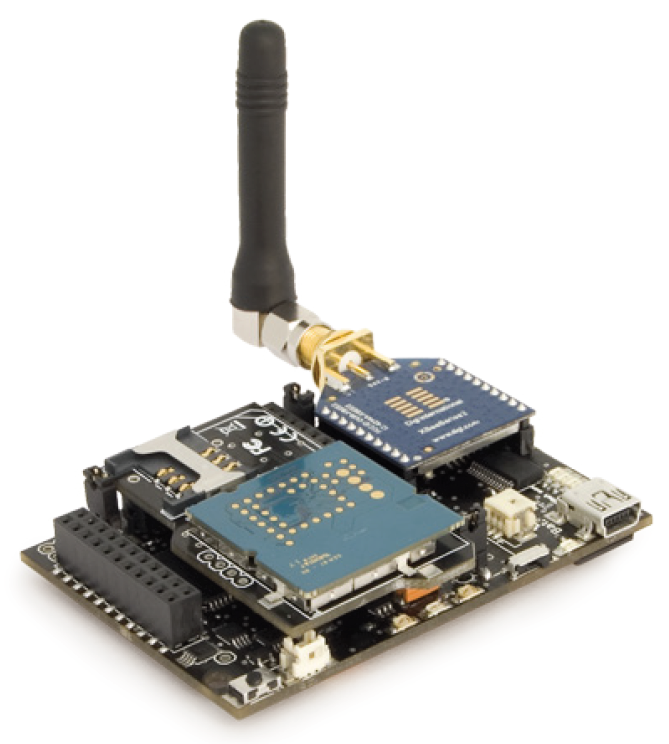
\includegraphics[height=6cm]{waspmote} \\[1.0cm] 

\begin{minipage}{0.4\textwidth}
\begin{flushleft} \large
\emph{Authors:}\\
{\authornames}
\end{flushleft}
\end{minipage}
\begin{minipage}{0.4\textwidth}
\begin{flushright} \large
\emph{Supervisor:} \\
{\supname}
\end{flushright}
\end{minipage}\\[2cm]

{\large \today}\\% Date

\vfill
\end{center}
\end{titlepage}

%----------------------------------------------------------------------------------------
%	REAL TITLE PAGE
%	Your institution may give you a different text to place here
%----------------------------------------------------------------------------------------

\addtocontents{toc}{\vspace{1em}} % Add a gap in the Contents, for aesthetics
\thispagestyle{empty}
\null\vfill 

\begin{center}
\Large{\textbf{DESIGN OF A WIRELESS SENSOR NETWORKING TEST-BED}}\\
\vspace{3cm}
\large{\emph{Bjorn Deraeve $\quad\bullet\quad$ Roel Storms}} \\
\HRule \\[1.0cm]
\vspace{1cm}
\normalsize{Written on behalf of Mr. Luc Vandeurzen}\\
\vspace{12cm}
{\large \today}
\end{center}

\vfill\vfill\vfill\vfill\

\clearpage % Start a new page

%----------------------------------------------------------------------------------------
%	QUOTATION PAGE
%----------------------------------------------------------------------------------------

%\pagestyle{empty} % No headers or footers for the following pages
%\null\vfill % Add some space to move the quote down the page a bit
%\textit{``Be a yardstick of quality. Some people aren't used to an environment where excellence is expected."}
%\begin{flushright}
%Steve Jobs
%\end{flushright}
%\vfill\vfill\vfill\vfill\vfill\vfill\null % Add some space at the bottom to position the quote just right
%\clearpage % Start a new page

%----------------------------------------------------------------------------------------
%	ABSTRACT PAGE
%----------------------------------------------------------------------------------------

\addtotoc{Abstract} % Add the "Abstract" page entry to the Contents

\abstract{\addtocontents{toc}{\vspace{1em}} % Add a gap in the Contents, for aesthetics

\emph{Audio applications are on of the main subfields of digital signal processing. More specific, in audio and music one can use frequency modulation synthesis in order to make creative and totally different sounding tones. A theoretical background and practical approach with an Analog Devices DSP-board is reported here.\\ \\
In the first two chapters it is explained how sound works and what aspects of frequency modulation are actually responsible for making a particular tone sound differently. Next a practical approach to add envelopes and effects to the tone is given.\\ \\
Chapter \ref{Chapter5} serves as introduction to \ref{Chapter6}. In this chapter some theoretical background and electronic designs of CPU architectures are explained. This chapter serves as a backbone for the practical implementations explored in chapter \ref{Chapter6}. Readers with a basic knowledge on this matter can skip this chapter and immediately start with chapter 6. The first part of this chapter handles the Analog Devices ADSP-21369 DSP board's initialisation routines and the second part focusses on the practical implementation of the signal creation and modulation algorithms.\\ \\
Finally chapter \ref{Chapter7} deals with the communication between the DSP-board and the Labview interface for the FM Synthesizer.\\ \\
As a conclusion chapter \ref{Chapter8} closes this report with some critical reflections on the implementation and team activities.}
}

\clearpage % Start a new page

%----------------------------------------------------------------------------------------
%	ACKNOWLEDGEMENTS
%----------------------------------------------------------------------------------------

%\setstretch{1.3} % Reset the line-spacing to 1.3 for body text (if it has changed)
%\acknowledgements{\addtocontents{toc}{\vspace{1em}} % Add a gap in the Contents, for aesthetics
%The acknowledgements and the people to thank go here, don't forget to include your project advisor\ldots
%}
%\clearpage % Start a new page

%----------------------------------------------------------------------------------------
%	LIST OF CONTENTS/FIGURES/TABLES PAGES
%----------------------------------------------------------------------------------------

\pagestyle{fancy} % The page style headers have been "empty" all this time, now use the "fancy" headers as defined before to bring them back

\lhead{\emph{Contents}} % Set the left side page header to "Contents"
\tableofcontents % Write out the Table of Contents

\lhead{\emph{List of Figures}} % Set the left side page header to "List of Figures"
\listoffigures % Write out the List of Figures

\lhead{\emph{List of Tables}} % Set the left side page header to "List of Tables"
%\listoftables % Write out the List of Tables

%----------------------------------------------------------------------------------------
%	ABBREVIATIONS
%----------------------------------------------------------------------------------------

\clearpage % Start a new page
\setstretch{1.5} % Set the line spacing to 1.5, this makes the following tables easier to read
\lhead{\emph{Abbreviations}} % Set the left side page header to "Abbreviations"
\listofsymbols{ll} % Include a list of Abbreviations (a table of two columns)
{
\textbf{RTC} & \textbf{R}eal \textbf{T}ime \textbf{C}lock \\
\textbf{CPU} & \textbf{C}entral \textbf{P}rocessing \textbf{U}nit \\

}

%----------------------------------------------------------------------------------------
%	PHYSICAL CONSTANTS/OTHER DEFINITIONS
%----------------------------------------------------------------------------------------

%\clearpage % Start a new page
%\lhead{\emph{Physical Constants}} % Set the left side page header to "Physical Constants"
%\listofconstants{lrcl} % Include a list of Physical Constants (a four column table)
%{
%Speed of Light & $c$ & $=$ & $2.997\ 924\ 58\times10^{8}\ \mbox{ms}^{-\mbox{s}}$ (exact)\\
%Constant Name & Symbol & = & Constant Value (with units) \\
%}

%----------------------------------------------------------------------------------------
%	SYMBOLS
%----------------------------------------------------------------------------------------

%\clearpage % Start a new page
%\lhead{\emph{Symbols}} % Set the left side page header to "Symbols"
%\listofnomenclature{lll} % Include a list of Symbols (a three column table)
%{
%$a$ & distance & m \\
%$P$ & power & W (Js$^{-1}$) \\
% Symbol & Name & Unit \\

%& & \\ % Gap to separate the Roman symbols from the Greek

%$\omega$ & angular frequency & rads$^{-1}$ \\
% Symbol & Name & Unit \\
%}

%----------------------------------------------------------------------------------------
%	DEDICATION
%----------------------------------------------------------------------------------------

\setstretch{1.3} % Return the line spacing back to 1.3
\pagestyle{empty} % Page style needs to be empty for this page
%\dedicatory{For/Dedicated to/To my\ldots} % Dedication text
\addtocontents{toc}{\vspace{2em}} % Add a gap in the Contents, for aesthetics

%----------------------------------------------------------------------------------------
%	CONTENT - CHAPTERS
%----------------------------------------------------------------------------------------

\mainmatter % Begin numeric (1,2,3...) page numbering

\pagestyle{fancy} % Return the page headers back to the "fancy" style
\setstretch{1.0}
% Include the chapters of the thesis as separate files from the Chapters folder
% Uncomment the lines as you write the chapters

% Chapter 1

\chapter{Sound nomenclature} % Main chapter title
\label{Chapter1} % To reference to this chapter elsewhere, use \ref{Chapter1} 
\lhead{Chapter 1. \emph{Sound nomenclature}} % This is for the header on each page - perhaps a shortened title
\textsf{\textsl{Written by Bjorn Deraeve}}
%----------------------------------------------------------------------------------------

\section{Introduction}
Sound is the human perception of little changes in air pressure. This oscillation of pressure, referred to as a sound wave, is a mechanical wave propagated through a solid, liquid or gas and is composed of frequencies within the range of hearing. For humans this is between about 20 Hz and 20 000 Hz, however the upper limit generally decreases with one's age.   The changes in pressure must also be big enough in order to be audible.

The mechanical vibrations interpreted as sound waves are longitudinal waves. Any source makes the matter in the medium periodically displace and thus oscillating. The alternating pressure deviations from the equilibrium pressure are in the same direction as the energy propagation of the wave. The energy carried by the wave is converted between potential energy (extra compression) and kinetic energy (oscillations of the medium).

When a sound wave reaches the eardrum it starts to oscillate at a frequency corresponding to the sound waves frequency. These vibrations are detected by hair cells in the inner ear and are transduced into nerve pulses (action potentials) which transmit information about the sound to the brain.

Sound waves are often described as sinusoidal waves which are characterized by a wavelength and amplitude. The wavelength is directly related to the frequency as $\lambda$ = $\frac{v}{f}$.  The higher the frequency, the higher the perceived tone will be. In dry air the speed of sound is approximately 343 meters per second. 

The sound wave causes a local pressure deviation from the ambient atmospheric pressure. To measure this deviation one uses the sound pressure level (SPL) scale. Since the human ear can detect sounds with a wide range of amplitudes (volumes) it is a logarithmic measure of the sound pressure at the deviation relative to a reference value. It is thus measured in an amount of decibels (dB) above the reference level. SPL is defined as:
\begin{equation}
L_{P} = 10\cdot \mathrm{log}_{10} (\frac{p^{2}}{p_{ref^{2}}} ) = 20 \cdot \mathrm{log}_{10} (\frac{p}{p_{ref}}) \medspace dB
\end{equation}
where p is the rms value of the measured sound pressure and pref is the reference sound pressure, pref = 20 microPa (rms), considered as the threshold of human hearing.
%----------------------------------------------------------------------------------------

\section{Sound characteristics}
A sound is defined by several characteristics. The most important are pitch (dutch: 'toonhoogte'), timbre (dutch: 'klankkleur') and are briefly introduced in this section. Other characteristics are volume and the duration of the rising of the sound, of the persistence and of the damping.
%----------------------------------------------------------------------------------------

\subsection{Pitch and tone}
For the human ear a pure tone is a sound with a constant frequency and timbre. This fundamental frequency, the number of perceived oscillations per second, is called the pitch of the sound. It is the frequency of the lowest tone present in the sound and is directly related to the frequency spectrum of the sound. Pitch allows the ordering of sounds on a frequency-based scale and is determined by the vibration frequency of the air. If air vibrations are not regularly there is no fixed frequency, such sound is called noise. On staves the pitch is indicated by the location of the note on the staff. The heigher the tone the higher the note is positioned on the staff.
\begin{figure}[htbp]
\centering
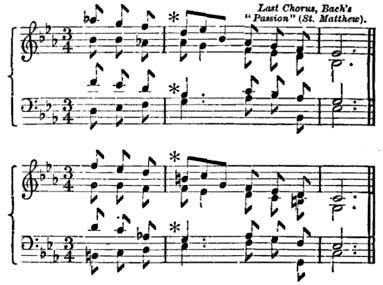
\includegraphics[height=5cm]{staff}
\rule{30em}{0.5pt}
\caption{Position of notes on staves}
\label{fig:staff}
\end{figure} \\
A tone with a double pitch is said to be one octave higher and is the first upper tone. In addition to the ordinary meaning of tone and pitch, in Western music theory tone is also the abstract term of future tones te sound, represented by the letters A to G and derived symbols (A = 440Hz). In some countries the fundamental tones are not indicated by letters but by the Greek diatonic scale (do-re-mi-fa-sol-la-si-do).
%----------------------------------------------------------------------------------------

\subsection{Timbre}
Timbre is the quality of a sound that distinguishes different musical instruments and voices. Timbre or tone colour is determined by the fundamental frequency (pitch) and the present overtones, also known as upper partials or harmonics, so timbre is composed of many different frequency components. It is determined by the ratio of the strength of the overtone vibrations in the sound in proportion to the fundamental frequency  of the sound.  

\subsubsection{Spectral diagram}
At this moment it is interesting to have a look at the spectral diagram of a sound. This diagram provides a link between the aural experience and visual representation of a sound. It does this by representing the energy (loudness, height of the line) and the frequency (position of the line) of the different frequency components within the timbre. It is unique to any sound and gives audible information about that sound. Waveforms are very descriptive for the way air pressure changes with time but not for the actual timbre of a sound.
\begin{figure}[htbp]
\centering
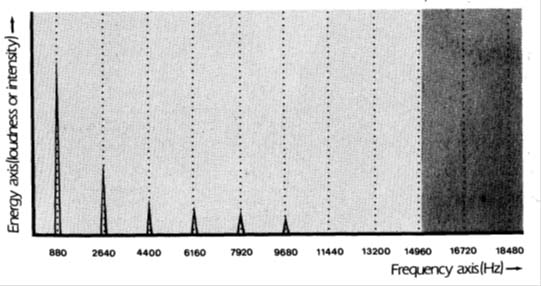
\includegraphics[height=5cm]{spectral}
\rule{30em}{0.5pt}
\caption{Spectral diagram of a timbre}
\label{fig:spectral}
\end{figure} \\
How can we interpret figure \ref{fig:spectral}? The line on the left is the fundamental frequency or first harmonic. The other frequencies visible in the spectrum, on the right of the first harmonic, indicate the other present frequencies in the sound. Most generally those are called 'partials'. If all partials are an integer multiple of the fundamental frequency they are called 'harmonics' or 'overtones' and the sound exists of the 'natural' harmonic frequencies only. \\ As we can see from the spectrum in figure \ref{fig:spectral}, the partials are in the harmonic series. The note played in this figure was A = 880Hz, this is the first harmonic. The next harmonic is at 3 times 880Hz or 2640Hz. This is the third harmonic, and so on. \\  From the relative height of the lines (representing the energy or loudness) we can deduce that the harmonics become weaker.
\subsubsection{Joseph Fourier}
Today when musicians desribe a timbre they talk about overtones, partials or harmonics, but it was the French mathematician and physicist Joseph Fourier who gave a mathematical basis to this idea with his work 'Th\'{e}orie de la chaleur" which he presented in 1822. In this investigation of the use of Fourier series for problems of heat transfer and vibrations, he brought up the following simplified statement: each complex sound, such as that from a violin or trumpet, can be thought of as the sum of a collection of much simpler tones (sines),  at frequencies which are an integer number multiples of the fundamental frequency (pitch). In other words: each complex sound can be resolved into mixtures of sine functions which may differ in amplitude and period but of which all periods are related as an integer multiple. This resolving into different components is called a Fourier transformation or analysis of the signal. \\ The spectrum as in figure \ref{fig:spectral} shows clearly the present frequencies (= partials, overtones or harmonics) and their energy level.
\begin{figure}[htbp]
   \centerline{\hbox{
   \epsfxsize=1.2in
   \epsffile{/fourier.jpg}
     }
  }
  \caption{Sketch of Fourier}
  \label{fig:fourier}
\end{figure}


%----------------------------------------------------------------------------------------
\section{ZigBee}
%----------------------------------------------------------------------------------------
\subsection{ZigBee standard}
%----------------------------------------------------------------------------------------
At the moment ZigBee is the leading protocol to implement low-cost low-data-rate, short-range WSNs. It is an open global standard built on IEEE 802.15.4 and provides extra functionality regarding advanced routing capabilities and network stability.
%-----------------------------------------
\subsection{ZigBee stack}
A common concept used to simplify and make digital communication more flexible, is the use of networking layers. Each layer is responsible for certain specific functions and pass data and commands only to the layers directly above or below via service access points. Figure \ref{fig:stack} shows how this is organized in the ZigBee protocol stack.  The bottom two layers are defined by the IEEE 802.15.4 standard and define the specifications for PHY and MAC layers. ZigBee only defines the networking, application and security layer on top of IEEE 802.15.4.\\
\begin{figure}[htbp]
\centering
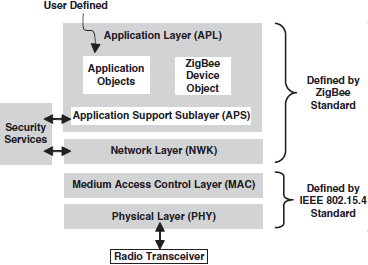
\includegraphics[width=0.48\textwidth]{stack}
%\rule{30em}{0.5pt}
\caption{ZigBee Protocol Layers}
\label{fig:stack}
\end{figure} 
\paragraph{PHY Layer Responsibilities}
\begin{itemize}
\item Enabling and disabling the radio transceiver ... ...
\item Transmit and receive data ... ...
\item Select CH ... ...
\item Estimating signal energy ... ...
\item Providing RSSI, LQI ... ...
\end{itemize}
\paragraph{MAC Layer Responsibilities}
\begin{itemize}
\item Generating beacons ... ...
\item CSMA-CA, BPSK vs. O-QPSK, vs. ASK ... ...
\item Providing a reliable link ... ...
\item PAN association and disassociation services
\end{itemize}
\paragraph{Network Layer Responsibilities}
\begin{itemize}
\item Setting up a network ... ...
\item Allow joining and leaving a network ... ...
\item Configuring new devices ... ...
\item Discover and maintain routes ... ...
\end{itemize}
\paragraph{Application Layer Responsibilities}
\begin{itemize}
\item Application support ... ...
\item Address management and mapping ... ...
\item Define the role of the device ... ...
\item Security related tasks ... ...
\end{itemize}
%-----------------------------------------
\subsection{Networking concepts}
\subsubsection{Device Types}
\subsubsection{Device Roles}
\paragraph{Coordinator Operation}
\paragraph{Router Operation}
\paragraph{End Device Operation}
sleep...
\subsection{Parent - Child relationship}
%-------------------------------------------------------------------
\subsection{API Frame Specifications}
To communicate with the ZigBee radio there are 2 modes, AT (transparent mode) and API (application programming interface). AT mode means that what you send to the zigbee radio using RS232, the ZigBee radio will send to its default destination. Unless you send “+++”, wait for the ZigBee to reply with OK, and then send an AT command. AT commands are used to change the configuration of the ZigBee radio. For instance the AT command OP requests the operating PAN ID.\\
AT mode is fairly limited and only good for point to point communication since you can’t really specify the destination unless you change the default destination all the time. So that is why the sensor network operates in API mode. This means that everything sent to the zigbee radio, using serial communication, is now packetized.\\
API defines a number of different packets as can be found in chapter 9 of \defcitealias{XBEE}{XBee/XBee-Pro ZB RF Modules User Manual, 2012}\citepalias{XBEE}. An API packet is shown in figure \ref{fig:api}. It starts with 0x7E as start delimiter and is followed by the length of the data excluding checksum. Then a API-specific structure follow which depends on the type of packet.\\
\begin{figure}[htbp]
\centering
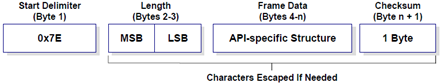
\includegraphics[width=0.48\textwidth]{api}
\caption{UART Data Frame Structure}
\label{fig:api}
\end{figure} 
\begin{table}[!ht]
\begin{center}
\begin{tabular}[!ht]{|c|c|}
\hline
\textbf{API Frame Name} & \textbf{API ID}\\
\hline
AT Command & 0x08\\
\hline
ZigBee Transmit Request & 0x10\\
\hline
AT Command Response & 0x88\\
\hline
ZigBee Receive Packet & 0x90\\
\hline
\end{tabular}
\caption{API Frame Names and Values}
\label{tab:apis}
\end{center}
\end{table}\\
\label{api1}\noindent
A reduced list of possible packets can be found in table \ref{tab:apis} (for the full list please see appendix \ref{AppendixF}). As mentioned an AT command is used to alter configurations of the ZigBee radio. This can of course also be done in API mode. For details about all the packets, please consult the datasheet. The only packets types used in this project are: 'ZigBee transmit request, 0x10' and 'Zigbee receive packet, 0x90'.\\
A ZigBee transmit request is shown in figure \ref{fig:api4}. This packet is used to send data from this ZigBee radio to a remote one. All that has to be known is the remote ZigBee address. These types of packets are constructed by the gateway to send out data to the libelium nodes but also by libelium nodes to send data to other libelium nodes or the gateway. Libelium has its own specific format for the RF Data as will be explained in section \ref{libPAQ}. To reach the gateway the address of the coordinator can be used, since the coordinator and gateway in our case are the same. This is convenient since the coordinator can always be addressed with 0x0000000000000000. The reason we chose the gateway and coordinator to be the same is that the coordinator receives a lot of traffic due to its role as coordinator and the same goes for the gateway. So these 2 devices should be in the center of the network for efficiency reasons. Assigning one device for these 2 roles and trying to position this device as central as possible will ask for the least amount of routing overhead.\\
When data is received by a ZigBee radio, this radio will send out a Zigbee receive packet via its serial communication. An example of this packet can be found in figure \ref{fig:api5}. Again the received data has an additional format as specified by Libelium.
\vfill  
% Chapter 3
\chapter{A WSN with Waspmotes: Theoretical aspects} % Main chapter title
\label{Chapter3} % For referencing the chapter elsewhere, use \ref{Chapter1} 
\lhead{Chapter 3. \emph{A WSN with Waspmotes: Theoretical aspects}} % This is for the header on each page - perhaps a shortened title


\section{Introduction}
Waspmote is more than just another piece of hardware. In fact it is an open source platform for wireless sensors, specially focusing on low consumption and autonomy. Waspmotes promise to offer a variable lifetime between 1 and 5 years, depending on the duty cycle and the used radio.\\ 
But it didn't just start with Waspmote and it will definitely not end with it. In 2007 developers from Libelium collaborated with the Arduino Team creating the first open hardware shield for Arduino, the "Arduino XBee Shield". The shield allowed an Arduino board to communicate wirelessly via ZigBee. Libelium used the shield to develop their first sensor device, the SquidBee, intended for creating sensor networks. Although the SquidBee is self-powered and implements wireless communications, it is more sensor device than wireless sensor device. The 3.3V - 5V regulator could not be turned off, as a result there is a constant consumption of 50mA discharging the battery within hours. The SquidBee was created for teaching and educational purposes only. Since the platform was not radio certified the motes could not be deployed in real scenarios like cities, factories or even houses, so it did not fit Libelium's corporate customer requirements at all. However, the tone of an open hardware and source wireless sensor device was definitely set.
\begin{figure}[ht]
  \hfill
  \begin{minipage}[t]{.45\textwidth}
    \begin{center}  
      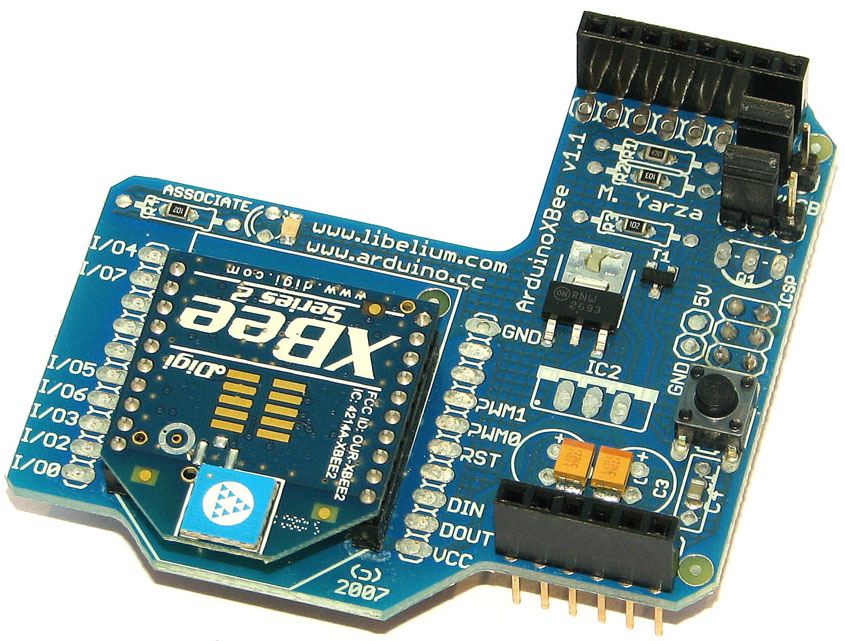
\epsfig{file=arduinoShield1, scale=0.20}
      \caption{Arduino XBee Shield}
      \label{fig:arduinoShield}
    \end{center}
  \end{minipage}
  \hfill
  \begin{minipage}[t]{.45\textwidth}
    \begin{center}  
      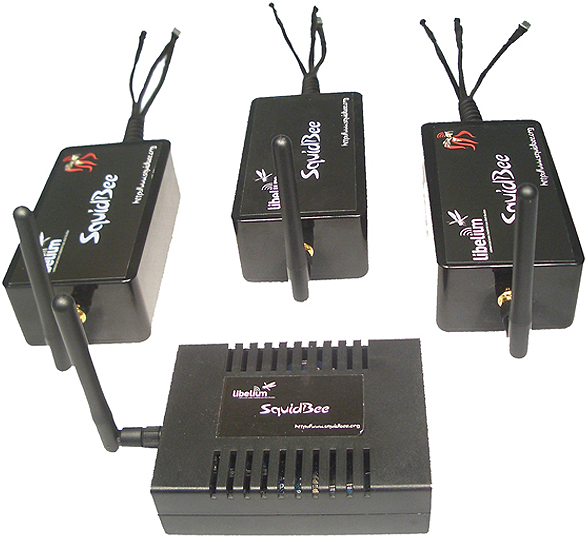
\epsfig{file=squidbee, scale=0.25}
      \caption{Libelium SquidBee}
      \label{fig:squidbee}
    \end{center}
  \end{minipage}
  \hfill
\end{figure}\\
In 2009 the Waspmote was born, meeting all the above requirements: low consumption and meeting three radio certification requirements (CE for Europe, FCC for the US and IC for Canada). In addition the Waspmote was built with a complete modular philosophy. The idea behind this design is to integrate only the needed modules in each device, optimizing costs. This is why all modules are connected to the Waspmote via sockets.\\Since its introduction, more than 2000 developers have been using Waspmote (v1.1) and the platform has received many suggestions and possible improvements. Libelium carefully listened to all these proposals and decided to bring out a new version with the name of Waspmote PRO (v1.2) in February 2013. This new version comes with upgraded hardware and an improved API, which is unfortunately not compatible with the older API. The most important improvements of the hardware is that the code can be uploaded much quicker and the XBee radio must no longer be removed, which is a huge improvement. There are also no more jumpers and there is no need of a coin battery. Regarding the API, Libelium claims it is much more robust and easier to use than the previous one and they also improved their programming guides. 
\begin{figure}[ht]
  \hfill
  \begin{minipage}[t]{.45\textwidth}
    \begin{center}  
      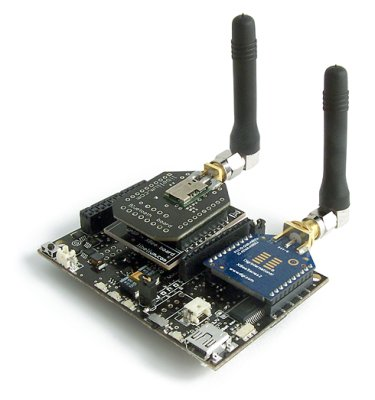
\epsfig{file=waspmote3, scale=0.45}
      \caption{Waspmote V1.1 with Bluetooth expansion module }
      \label{fig:arduinoShield}
    \end{center}
  \end{minipage}
  \hfill
  \begin{minipage}[t]{.45\textwidth}
    \begin{center}  
      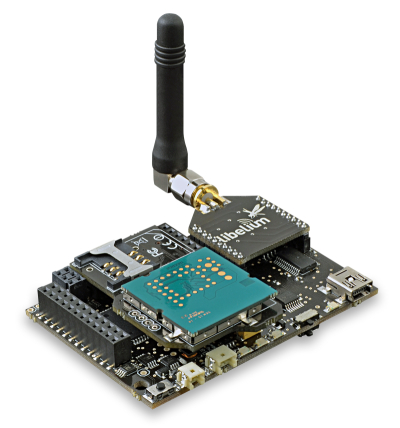
\epsfig{file=waspmotePro, scale=0.40}
      \caption{Waspmote PRO}
      \label{fig:squidbee}
    \end{center}
  \end{minipage}
  \hfill
\end{figure}\\   
%----------------------------------------------------------------------------------------
\section{Hardware}
\subsection{Modular Architecture}
As mentioned in this chapter's introduction, Waspmote is based on a modular architecture, doing so optimizing costs and able to change according to the specific user's requirements. The available modules are split up into five categories:
\begin{itemize}
\item ZigBee
\item GSM - 3G/GPRS
\item GPS
\item Sensor Boards
\item Storage
\end{itemize}  
Figure \ref{fig:waspMote1} indicates the Waspmote main components.
\begin{figure}[ht]
\centering
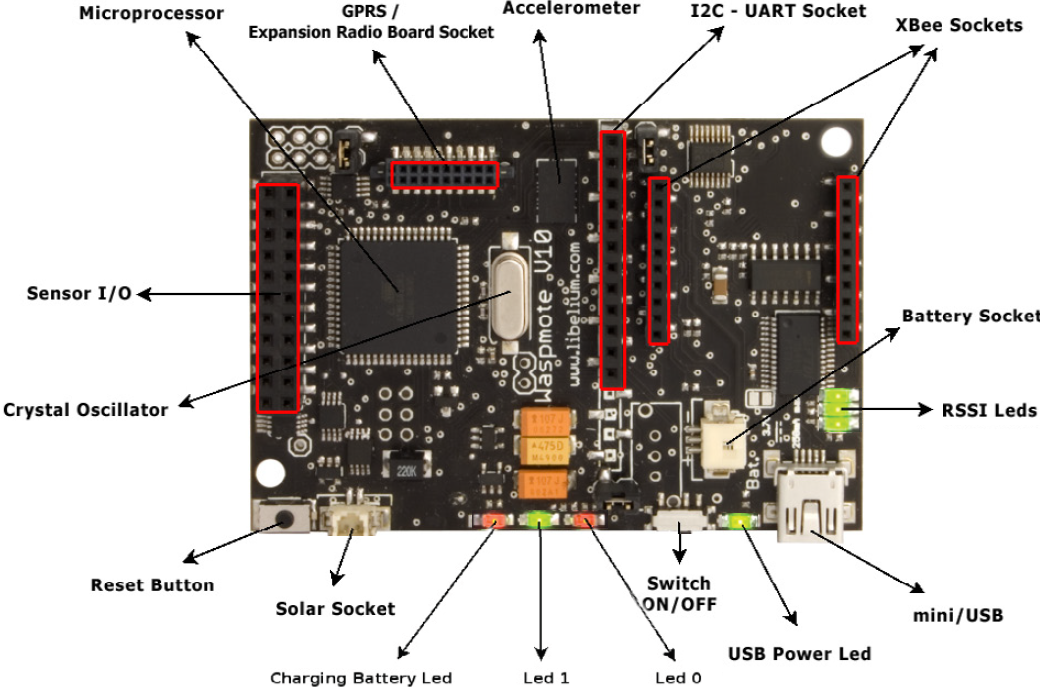
\includegraphics[height=6.5cm]{waspmote2}
\rule{30em}{0.5pt}
\caption{Main Waspmote components}
\label{fig:waspMote1}
\end{figure}
%-------------------------------------------
\subsection{Microcontroller and memory}
Just like on any other PCB, the CPU is the heart of the module. Waspmote integrates an 8-bit ATmega 1281 microcontroller with 128KB programmable flash, 8KB SRAM runtime memory and 4KB EEPROM memory. Since SRAM is is built with cleverly combined MOSFETs it must not be periodically refreshed, but it is still volatile memory. The main advantage compared to DRAM is that, when moderately clocked like in the Waspmote, it consumes very little power.\\
Because of the modular design of the Waspmote the block diagram is very simple. This is shown in figure \ref{fig:block}.
\begin{figure}[ht]
\centering
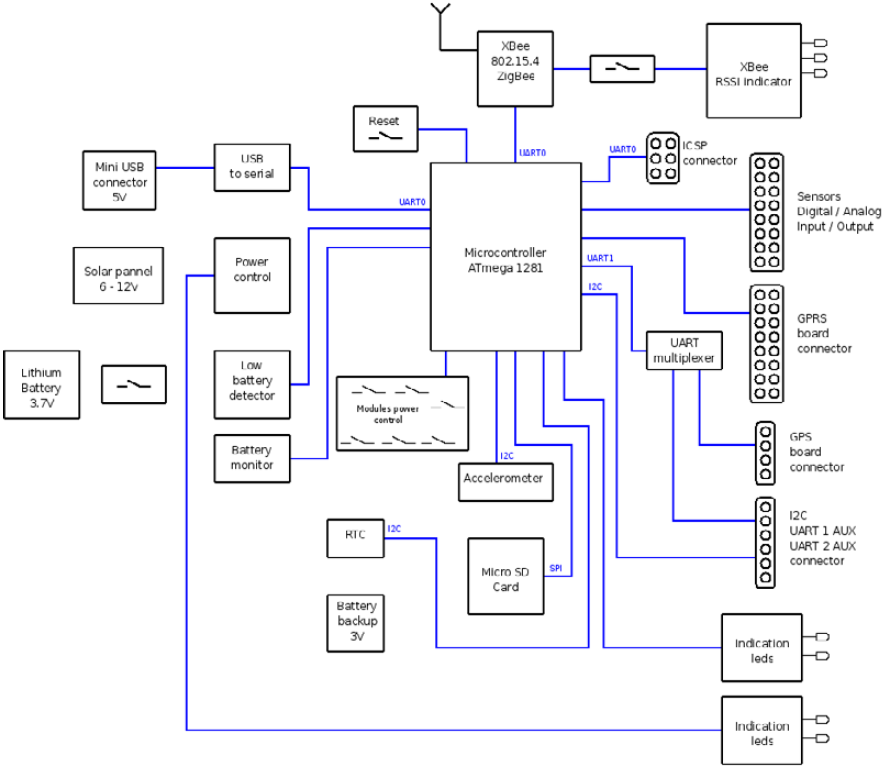
\includegraphics[height=11.5cm]{block}
\rule{30em}{0.5pt}
\caption{Waspmote block diagram}
\label{fig:block}
\end{figure}
%-------------------------------------------
\subsection{Timers}
The Waspmote's system clock is an 8MHz quartz oscillator. This means that every 125ns a machine language instruction is executed by the microcontroller. Keep in mind that one C++ instruction consists of several instructions in machine language. To generate interrupts the Waspmote has an internal watchdog and a Real Time Clock (RTC).
\subsubsection{Watchdog}
The Watchdog is integrated on the Atmega 1281 and counts the clock cycles generated by a 128KHz oscillator. When the WDT counter reaches a set value it generates an interruption signal. The WDT is used to awake the microcontroller from \textit{Sleep} mode, because of its high precision. Thus, \textit{Sleep} mode allows small intervals, going from 16 milliseconds to a maximum of 8 seconds.
\subsubsection{Real Time Clock}
To store an absolute time base the RTC can be used. Alarms programmed in the RTC specify days, hours, minutes and seconds. For the RTC the waspmote uses a Maxim DS3231SN 32.768Hz oscillator. Because this clock has an internal compensation mechanism for variations caused by temperature changes this is one of the most accurate clocks on the market. This clock is used to wake the Waspmote from the higher energy saving modes \textit{Deep Sleep} and \textit{Hibernate}, with intervals from 8 seconds to even days. It is important to notice that in \textit{Hibernate}, the RTC is no longer powerd through the main battery but through the auxiliary (button) battery. So when problems occur when using hibernate probably it is recommended to measure the button battery's voltage and possibly must be replaced.
%----------------------------------------------------------------------------------------
\section{Programming}
To develop on the Waspmote, Libelium offers an API and IDE. For more information on the API, please see chapter \ref{Chapter4}. Waspmote uses the same IDE (compiler and core libraries) as Arduino, so as long as things like pin layout and I/O schemes are adjusted, code should be compatible in both platforms. So Waspmote and Arduino are pretty much the same, however don't forget that Waspmote has Radio Certifications and Arduino doesn't.\\  
When the Waspmote is started, the microcontroller will execute the bootloader and start loading the compiled program from FLASH into the SRAM working memory.\\
The code is divided into two basic parts: \textbf{setup} and \textbf{loop}, each with sequential behaviour. When the Waspmote is switched on or reset, the code starts at the setup function and then enters the loop function. Because the second part forms an infinite loop a common technique to save energy is to block the program until some interruption is detected.\\
Since in \textit{Hibernate} mode the Waspmote is completely disconnected from the main battery also the program is interrupted. This means the SRAM has lost all variable values and at wake up the code restarts at the \textbf{setup} function. To store values during hibernate cycles it is necessary to write them to EEPROM or the SD card.
%----------------------------------------------------------------------------------------
\section{Power considerations}
\label{pow}
\subsection{Waspmote power modes}
The libelium Waspmote has 4 operational modes: ON, Sleep, Deep Sleep and Hibernate. They differ from which type of interruptions they can be woken up and duration interval. For our application we want sleep intervals of 30 seconds and more, so only Deep Sleep and Hibernate mode are of interest. Table \ref{tab:cons1} summarizes the Waspmotes operational modes.
\begin{table}[!ht]
\begin{center}
\begin{tabular}[!ht]{|c|c|c|c|c|}
\hline
\textbf{Mode} & \textbf{Consumption} & \textbf{CPU} & \textbf{Cycle} & \textbf{Accepted Interruptions}\\
\hline
ON & 9mA & ON & - & Synch and Asynch\\
\hline
Sleep & 62$\mu$A  & ON & 31ms - 8s & Synch (WDT) and Asynch\\
\hline
Deep Sleep & 62$\mu$A & ON & 8s - min/hours/days & Synch (RTC) and Asynch\\
\hline
Hibernate & 0.7$\mu$A & OFF & 8s - min/hours/days & Synch (RTC)\\
\hline
\end{tabular}
\caption{Operational modes of Libelium Waspmote V1.1}
\label{tab:cons1}
\end{center}
\end{table}
\subsubsection{Deep Sleep}
In deep sleep mode the main program is paused and the CPU passes to a latent state. Triggers are as well synchronous interruptions (RTC) as asynchronous interruptions. Examples of asynchronous interruptions are low battery level or a sensor that reaches a certain trigger value.\bigskip
\begin{figure}[ht]
\centering
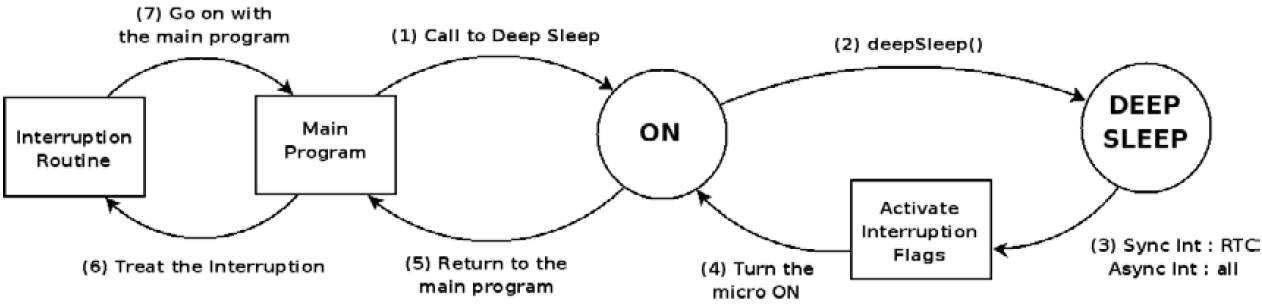
\includegraphics[height=3cm]{deepSleep}
\rule{30em}{0.5pt}
\caption{Waspmote going from ON to Deep Sleep}
\label{fig:deepSleep}
\end{figure}\bigskip
\\In figure \ref{fig:deepSleep} the process from going to operational mode ON to Deep Sleep is shown. The main advantage of this mode is that the program is only paused, so the program stack and thus all variable values keep their values. When the Waspmote is turned back on it simply executes the next instruction.
%-------------------------------------------
\subsubsection{Hibernate}
Hibernate mode consumes roughly 100 times less energy than Deep Sleep. This is made possible by disconnecting all the Waspmote's modules, including the microcontroller. The RTC gets his power through the auxiliary battery. So if hibernate mode stops working it is probably necessary to replace the Waspmote's button battery. Figure \ref{fig:hibernate} demonstrates the process from ON to hibernate.\\
\begin{figure}[ht]
\centering
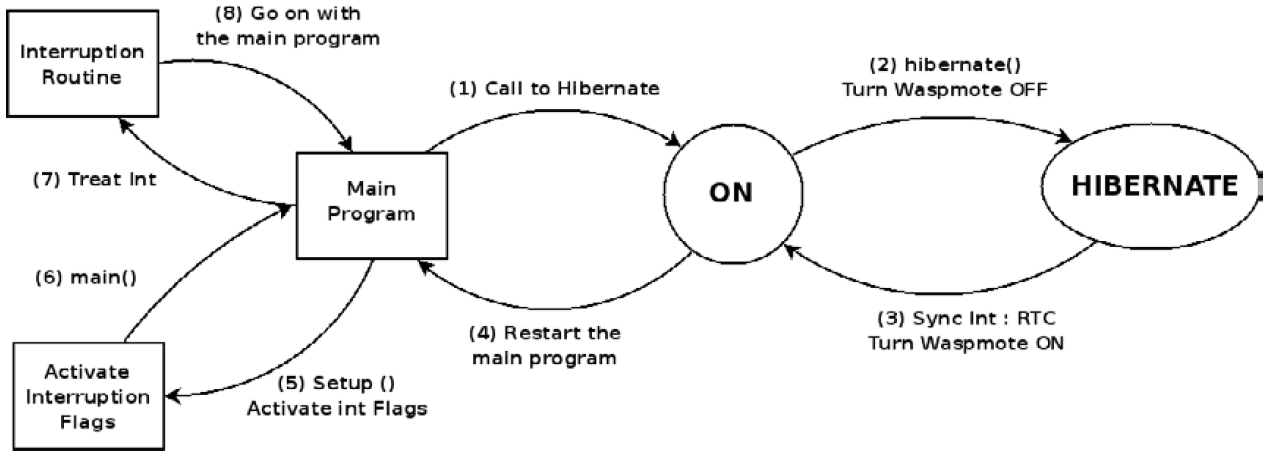
\includegraphics[height=4.5cm]{hibernate}
\rule{30em}{0.5pt}
\caption{Waspmote going from ON to Hibernate}
\label{fig:hibernate}
\end{figure}
This means the CPU is also switched of and does not remember any values from variables. When waking up the Waspmote reinitializes, the microprocessor is reset and the program restarts from the beginning. Both \textbf{setup} and \textbf{loop} routines are executed as if the main switch would be activated. By placing the \verb+ifHibernate()+ function in setup the program can determine if it came from a hardware reset or from a hibernate reset. To be able to wake up from hibernate mode the hibernate jumper must be removed correctly. See section .... for remarks on this issue. \\Because not all Libelium's API functions regarding hibernate in combination with the different alarm modes work, it is advised to use the functions provided in \textbf{WaspXBeeZBNode.h}. 
%----------------------------------------------------------------------------------------
\subsection{Sampling sensors}
To measure the sensors, originally we took 10 samples with 100 milliseconds recommended delay between the measurements and calculated the average. Since we want to make the energy consumption as low as possible we now do the iterations without delay. Appendix \ref{apendixSensorSensitivity} contains 60 test samples per sensor and indicates that there is no significant difference on the average by removing this delay. Except for CO$_{2}$ measurements, removing the delay saves about 1000 milliseconds per measured sensor.\\ 
Because the first sample often shows a slight deviation, the program takes 11 samples but bases the average on the last 10 values.
%-------------------------------------------
\subsection{Battery life estimation}
In order to be able to give recommended sensor measuring intervals this section will analyse the estimated battery life of the Waspmotes. Table \ref{tab:cons2} enumerates the most common components typical consumption.
\begin{table}[!ht]
\begin{center}
\begin{tabular}[!ht]{|c|c|}
\hline
\textbf{Action} & \textbf{Average Current}\\
\hline
XBee, sending, & 105mA\\
\hline
CO$_{2}$ & 50mA\\
\hline
XBee, ON & 45mA\\
\hline
Waspmote, ON & 9mA\\
\hline
Pressure & 7mA\\
\hline
Humidity & 380$\mu$A\\
\hline
Waspmote, sleep & 62$\mu$A\\
\hline
Temperature & 6$\mu$A\\
\hline
Waspmote, hibernate & 0,007$\mu$A\\
\hline
\end{tabular}
\caption{Operational modes of Libelium Waspmote V1.1}
\label{tab:cons2}
\end{center}
\end{table}
The batteries included with our Waspmotes are rechargeable Lithium-ion batteries with a capacity of 6600mAH. The Waspmote that will be deployed on the roof of Group T, campus Vesalius will also have a 12V solar panel with a charging current up to 280 mA to extend its battery life. The other batteries can by charged manually or by USB (5V, 100mA). Lithium-ion have a self-discharge rate of typcially 1 to 2 percent per month and since the used batteries are new we expect a high battery efficiency.\\
%-------------------------------------------
\subsubsection{XBee and Waspmote start-up times}
For the XBee node to join an existing network there are two power related possibilities. Either the Waspmote has been turned on already sufficiently long and the XBee had more than enough time to join the network, or either the XBee wasn't joined yet and the program needs to wait on this. From the experiments done at our apartment we came to following conclusions:
\begin{enumerate}
\item It takes about 2.5 seconds to join a network after powered on.
\item If the XBee is joined, the program still needs to confirm this. This takes 452 milliseconds.
\item The sending time is constant, about 158 ms, if the XBee had more than 2.5 seconds to join. However in case the XBee must send immediately after it is joined, the sending time is not constant and takes on average 611 milliseconds.
\item The sending time increases if there are more obstructions between the antennas. 
\end{enumerate}
With these characteristics we came to results discussed in the next sections. For the validation of these conclusions please see appendix \ref{AppendixA}. Table \ref{tab:sendTime} sums up the results of the distance-relation test.
\begin{table}[!ht]
\begin{center}
\begin{tabular}[!ht]{|c|c|}
\hline
\textbf{Distance} & \textbf{Average sending time (ms)}\\
\hline
Air & 158\\
\hline
1 Floor & 268\\
\hline
2 Floors & 357\\
\hline
3 Floors & 484\\
\hline
4 Floors & 558\\
\hline
5 Floors & unreachable\\
\hline
\end{tabular}
\caption{Distance consequence on send times}
\label{tab:sendTime}
\end{center}
\end{table}\\
To save power the Waspmote can store the values for a user determined time. Taking samples and save them to EEPROM in case of hibernate mode takes only 6 - 7\% of the time to measure and send. Table \ref{tab:sendTime3} confirms this.
\begin{table}[!ht]
\begin{center}
\begin{tabular}[!ht]{|c|c|}
\hline
\textbf{Nr of samples per sensor} & \textbf{Average ON time (ms)}\\
\hline
10 & 210\\
\hline
3 & 194\\
\hline
\end{tabular}
\caption{Time needed to sample and store 4 sensors}
\label{tab:sendTime3}
\end{center}
\end{table}
%-------------------------------------------
\subsubsection{Battery life with standard program optimizations}\label{batLife1}
The application scenario for this battery test is as follow: the Waspmote will be turned on as short as possible and 4 sensors, namely temperature, humidity, pressure and battery level will be sampled. The node will take 10 samples for each sensor and calculate the average. Those values are put into one ZigBee packet and sent to the gateway. By adapting the sleep time between the event we came to the rather disappointing results shown in figure \ref{fig:batCalcHP}.\\ The graph in figure \ref{fig:batCalcHP1} breaks down the total energy consumption to five categories. It shows the monthly energy consumption as a function of the time between the events. For small intervals the active energy usage is huge. Only starting at 20 minutes sleep time the self-discharge becomes dominant and from 3 hours on the sleep mode current also becomes dominant.\\
Since the Waspmotes use this much energy when applied this way we will call this the High Performance mode from now on. The next section calculates an alternative approach, referred to as Power Saver mode. This nomenclature is continued in the program:
\begin{alltt}
    typedef enum \{HIGHPERFORMANCE, POWERSAVER\} PowerPlan; 
\end{alltt}
\begin{figure}[htbp]
\centering
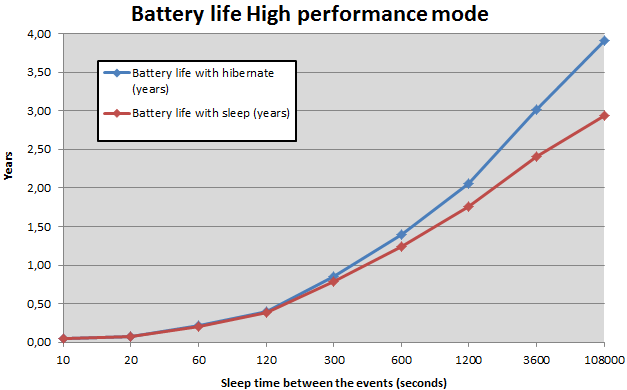
\includegraphics[height=8.5cm]{batCalcHP}
\rule{30em}{0.5pt}
\caption{Battery life in High performance mode}
\label{fig:batCalcHP}
\end{figure}
\begin{figure}[htbp]
\centering
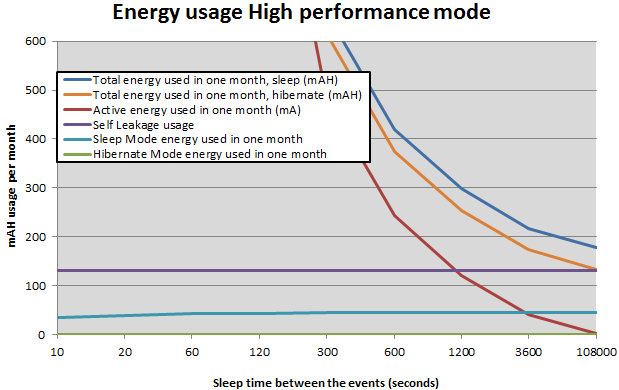
\includegraphics[height=8.5cm]{battery1}
\rule{30em}{0.5pt}
\caption{Energy usage in High performance mode}
\label{fig:batCalcHP1}
\end{figure}
Table \ref{tab:cons2} summarizes the battery duration in years of both performance and power saver mode.
\begin{table}[!ht]
\begin{center}
\begin{tabular}{cc|c||c|c|l}
\cline{2-5}
 & \multicolumn{2}{ |c|| }{Deep Sleep} & \multicolumn{2}{c}{Hibernate}\vline\\ \cline{1-5}
\multicolumn{1}{ |c| }{Sleep duration} & High Performance & Power Saver & High Performance & Power Saver    \\ \cline{1-5}
\multicolumn{1}{ |c| }{10s} & 0,05 & 0,92 & 0,05 & 1,00    \\ %\cline{1-5}
\hline
\multicolumn{1}{ |c| }{1min} & 0,21 & 2,15 & 0,21 & 2,63   \\ %\cline{1-5}
\hline
\multicolumn{1}{ |c| }{3min} & 0,79 & 2,75 & 0,85 & 3,59   \\ %\cline{1-5}
\hline
\multicolumn{1}{ |c| }{10min} & 1,25 & 2,85 & 1,39 & 3,76   \\ %\cline{1-5}
\hline
\multicolumn{1}{ |c| }{20min} & 1,75 & 2,90 & 2,06 & 3,85  \\ %\cline{1-5}
\hline
\multicolumn{1}{ |c| }{1h} & 2,41 & 2,94 &3,02 & 3,91    \\ %\cline{1-5}
\hline
\multicolumn{1}{ |c| }{3h} & 2,94 & 2,96 &3,90 & 3,94    \\ %\cline{1-5}
\hline
%\multicolumn{1}{ |c  }{\multirow{2}{*}{Powers} } &
%\multicolumn{1}{ |c| }{gcd} & 2 & 2 & 0 & 0 & min \\ \cline{2-6}
%\multicolumn{1}{ |c  }{}                        &
%\multicolumn{1}{ |c| }{lcm} & 3 & 3 & 1 & 1 & max \\ \cline{1-6}
\end{tabular}
\caption{Battery life in years for High Performance and Power Saver}
\label{tab:cons2}
\end{center}
\end{table}\\

%-------------------------------------------
\subsubsection{Battery life with extra optimizations}
As shown earlier in this section, sending values requires that the Waspmote is on for at least 3 seconds. In addition the XBee uses about five times the energy of the Waspmote. For end devices it is obviously recommended to turn on the XBee as little as possible, within a user defined limit.\\ Figure \ref{fig:batCalcPS} shows the same results as the application scenario discussed in section \ref{batLife1} and adds the results for a mode further referred to as Power Saver.\\
The implementation of this mode will depend on the nodes sleep settings. For \textit{Deep Sleep} the values can simply be stored on the heap, but for \textit{Hibernate} the values must be written to EEPROM.\\
Because of the size limit of a ZigBee packet we can store maximum 30 values and send them in one packet. However, if the sensor measuring interval is small the user can opt to store more values and send two or more packets after each other. The values for Power Saver in table \ref{tab:cons2} are of an example scenario that takes 60 measurements and then sends them in two packets to the gateway. It are also those results which are put in function of time in figure \ref{fig:batCalcPS}.\\

\begin{figure}[htbp]
\centering
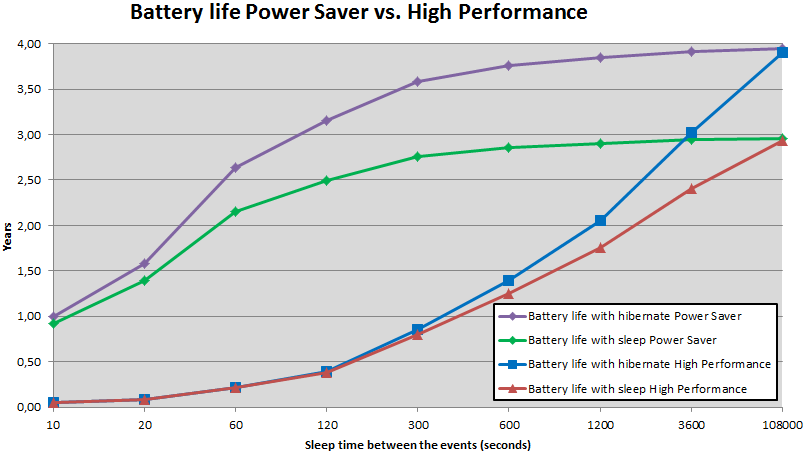
\includegraphics[height=8.5cm]{battery2}
\rule{30em}{0.5pt}
\caption{Battery life High Performance vs. Power Saver}
\label{fig:batCalcPS}
\end{figure}\bigskip
\begin{figure}[htbp]
\centering
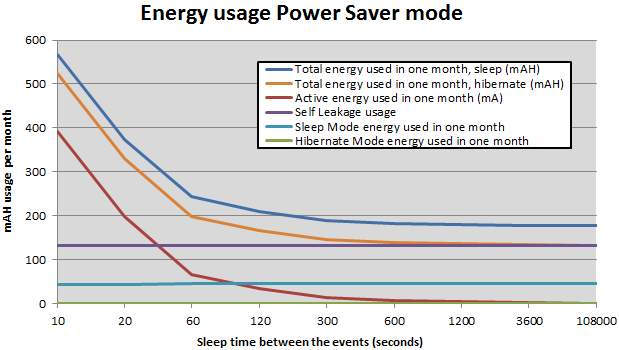
\includegraphics[height=8.5cm]{battery3}
\rule{30em}{0.5pt}
\caption{Energy usage in Power Saver mode}
\label{fig:batCalcPS1}
\end{figure}

As visible on figure \ref{fig:batCalcPS} \textit{Hibernate} has more influence in Power Saver mode, already extending battery life significantly at a 20 seconds interval comparing to a 10 minutes interval in High Performance mode. Also the energy breakdown graph in figure \ref{fig:batCalcPS1} shows that the interval times must be increased much less before the dominant factor is self-discharge and sleep mode energy consumption, compared to figure \ref{fig:batCalcHP1}.\\By reducing the sensor measurement accuracy battery life can be extended with modest 3 - 4\%, best case scenario. Please see appendix \ref{appendixA} for details.\\
In case the measuring intervals are small it is recommended to use \textit{Deep Sleep} instead of \textit{Hibernate}, since in hibernate the values are written to EEPROM. Equation \ref{eq:1} shows this can be very destructive for the Waspmote. Depending on how much freedom the user is given, the program can make the decision to switch to \textit{Deep Sleep} on itself, or the installation's administrator can control this.
% Chapter 4
%----------------------------------------------------------------------------------------
\section{A WSN with Waspmotes: Implementation aspects}
\subsection{Introduction}
\label{lab5}
In this section the program running on the WSN nodes will be discussed. To start programming, Libelium offers its customers a customized IDE\footnote{Integrated Development Environment (IDE)} and a fairly extensive API. The IDE uses the same compiler and core libraries as the Arduino IDE and is ideal to upload small examples and test programs to the nodes. However, to facilitate programming and to obtain more C/C++ support, expanding the API is required. This will be discussed in more detail in section \ref{LibAPI}.\\
After experimenting with the ZigBee sleep modes it became clear that the instability caused by delayed, pending messages for end devices could not be avoided. The program does support ZigBee sleep modes but this section will only discuss the \textit{stable operation modes without ZigBee sleep}. From now on, we will no longer differentiate between ZigBee routers and ZigBee end devices, but the sleep options will be controlled via Waspmote sleep modes, as recommended by Libelium \defcitealias{LIBSLEEP}{Libelium-dev, 2013}\citepalias{LIBSLEEP}. So a ZigBee router forced to sleep as well as a ZigBee end device will be considered an 'End Device'. 

%---------------------------------------------------

\subsection{Overall Program Structure}
\label{program}
When ZigBee sleep modes are ignored, basically three different programs suffice to program the entire network. There is one program to support the gateway (which is also the ZigBee coordinator) which analyses the data received from the other nodes, which is running on a Linux machine instead of a Waspmote. This will be discussed in section \ref{extracting}. All the nodes that collect sensor data are either running a 'Router' program or an 'End Device' program, which is designed to collect and send the sensor samples to the gateway. The only difference between these last two programs is that a 'Router' program does not implement sleep modes. The next sections will discuss the 'End Device' operation. A flowchart is shown in figure \ref{fig:flow}.\\
In a default program cycle each node has to associate with the network, measure some sensors, send the measured samples and possibly enter a sleep mode before repeating this cycle, depending on whether it has a 'Router' program or an 'End Device' program running.\\ 
\begin{table*}[htbp]
\begin{center}
\begin{tabular}[htbp]{|c|c|c|c|c|}
\hline
\textbf{Mode} & \textbf{Consumption} & \textbf{CPU} & \textbf{Cycle} & \textbf{Accepted Interruptions}\\
\hline
ON & 9mA & ON & - & Synch and Asynch\\
\hline
Sleep & 62$\mu$A  & ON & 31ms - 8s & Synch (WDT) and Asynch\\
\hline
Deep Sleep & 62$\mu$A & ON & 8s - min/hours/days & Synch (RTC) and Asynch\\
\hline
Hibernate & 0.7$\mu$A & OFF & 8s - min/hours/days & Synch (RTC)\\
\hline
\end{tabular}
\caption{The operational modes of Libelium Waspmote V1.1}
\label{tab:cons1}
\end{center}
\end{table*}
\begin{figure*}[htbp]
\centering
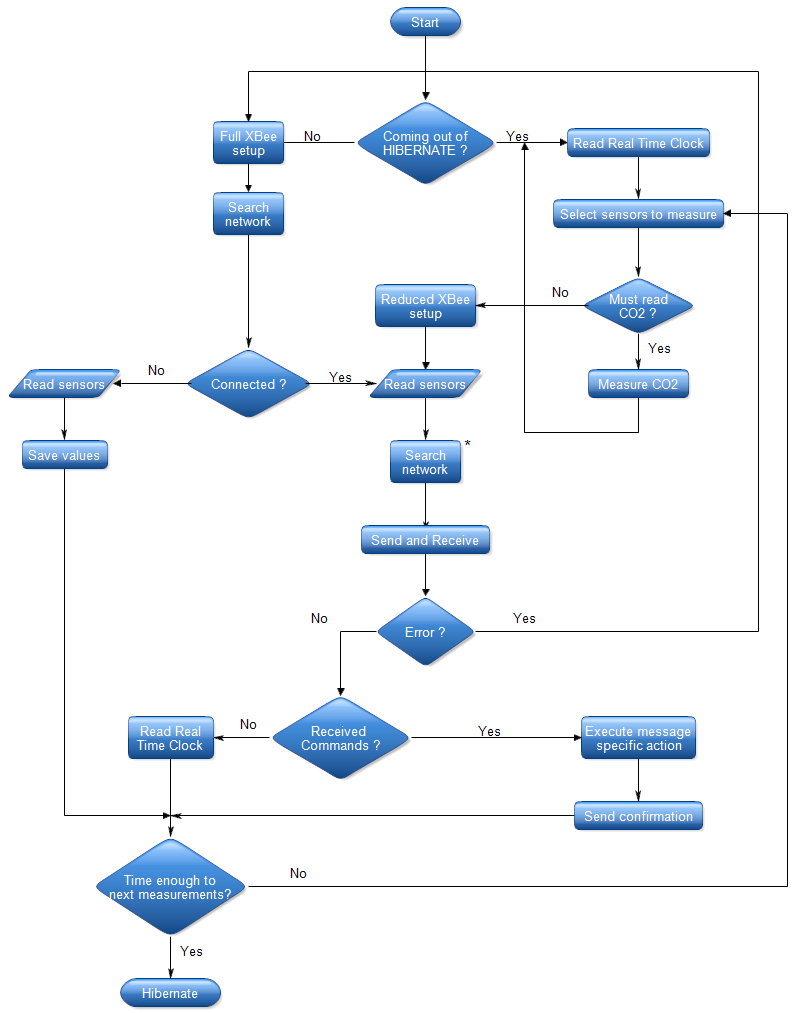
\includegraphics[height=19cm]{WSN2}
\caption{A flow chart of the Waspmote program for end devices}
\label{fig:flow}
\end{figure*}

\subsubsection{Initialization}
\label{initial}
\paragraph{Device start-up: Full initialization}
When the program is executed for the first time, a full XBee setup will be executed with the parameters retrieved from the program in the Libelium IDE. To ensure stability it takes about 8 seconds to write the settings to the XBee, to reset it afterwards (turn the power off and back on) and finally to perform the joining process. From this moment on the node will send its battery level to the coordinator and wait to receive an 'ADD\_NODE\_REQUEST' packet, containing its physical sensor layout settings, from the web interface. Until such a packet is received the node's sleeping time will gradually be increased.
\paragraph{Next cycles: Reduced initialization}
By not resetting the PAN ID but simply fetching it from the XBee's memory, the joining process only takes about two seconds\footnote{By enabling ZigBee sleep, the node does not lose the association with its parent and the re-joining process only takes about 10ms. However, the time needed to receive messages pending in router devices varies between 5 and 15 seconds and is never compensated by the faster joining process. There is also no guarantee that pending messages will be received or in which order they will be received, so network stability can no longer be guaranteed.} (Please see appendix \ref{timess} for more measurement results). Unfortunately a disadvantage of this shortened setup is that the XBee is no longer able to detect if the coordinator or his parent is actually available. The result of the executed association check is not always correct and the program will only notice this for the first time when it is trying to send a message. If this function results in a send error the program will do a full setup routine and resend the message. If the node then fails again to send the message we can conclude that the coordinator is really off-line or that there are no joinable nodes within range. In that case the message content will be saved and tried to be sent during the next cycles. In order not to lose the results, the gateway or web interface can keep track of the number of consecutive cycles a node has failed to report and notify a system administrator to avoid losing the saved values.

\subsubsection{Measuring sensors}
To sample a sensor from the expansion board, the Libelium API functions can be used. The functions return a float value corresponding to the sensor's measuring unit. Until an 'ADD\_NODE\_REQUEST' is received each node will measure its battery level and send it to the gateway. Via this packet the node gets to know its physical sensor layout and can decide if a future request of a sensor value is allowed.\\
%------------------------------
%\paragraph{Sample conversion}
To shorten messages (the ZigBee maximum payload is 74 Bytes \defcitealias{ZBGUIDE}{Waspmote ZigBee Networking Guide, 2012}\citepalias{ZBGUIDE} ) and to reduce transmission times, all values are sent in hexadecimal representation. This way all sensors fit within with 1 or 2 bytes. An example conversion is given for a temperature sample with two decimals:
\usestyle{vs} %other useful styles are, bw,  borland, vs
\includecode{tempConv.cpp}
%------------------------------

\subsubsection{Sending samples}
\label{frames1}
The API of Waspmote V1.1 introduces an 'Application Header' (see figure \ref{fig:appH} ) to send and receive data. This header takes care of packet fragmentation if packets exceed the maximum payload limit and can also be used by the receiver to treat the packet or fragment. The header itself is sent inside the RF Data field of the API Frame Structure, which was discussed in more detail in section \ref{ZBStructure} (see figure \ref{fig:frames}).
\begin{figure}[ht]
\centering
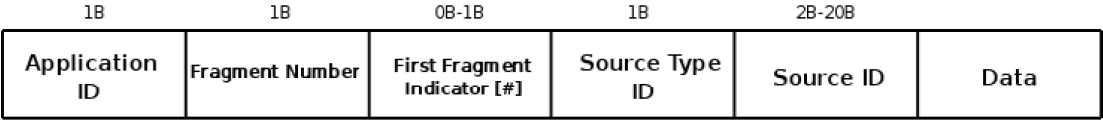
\includegraphics[width=0.48\textwidth]{appHeader}
\caption{The application Header}
\label{fig:appH}
\end{figure}\\
\noindent
The Waspmote and gateway programs use the 'Application ID' field in this header to distinguish different data packets. This extra layer also serves as an acknowledgement in the communication protocol. Depending on the 'Application ID' the layer contains a sensor mask (a 16 bit-flag) and data. With uniform timing settings, when a node awakens, it will measure the sensors found in its 'activeSensorMask' and send them to the gateway via an 'IO\_DATA' packet. This packet will be indicated as 'IO\_DATA' via the 'Application ID' field and will contain the mask of the measured sensors followed by their corresponding values.\\
To easily process this mask all sensor types are stored as follows:
\usestyle{vs} %other useful styles are, bw,  borland, vs
% Include the source code 
\includecode{sensType.cpp}
The sensor mask of a packet as well as the active mask stored in a certain node is a 16-bit value in which each bit indicates if a sensor must be taken into account or not.

%------------------------------
\paragraph{Escaping zeros}
Before sending the hexadecimal values all zeros must be removed (zeros are interpreted as end of string characters). Zeros will be replaced by \verb+0xFFFE+, so an extra byte is necessary. \verb+0xFF+ is the chosen escape character and \verb+0xFE+ is added to distinguish between an escaped zero and the value \verb+0xFF+ itself. The escaped character itself is of course also escaped.
\paragraph{Constructing packets}
To easily introduce the sensors into the packet to be sent, the program uses static function pointers. Part of the code to insert the measured sensors into an 'IO\_DATA' packet is given below. All Waspmote functions with error checking start with \verb+uint8_t error = 2+. If the returned error equals 2, the function has not been executed. Whereas 1 means something went wrong and 0 indicates a success. Each function pointer knows the size of the sample and updates the \verb+pos+ variable, which determines the location of the sample in the 'IO\_DATA' packet. This size and thus position depends on which sensor is included into the packet. The first two bytes of this packet are reserved for the sensor mask, indicating which sensor values are following. For example, an 'IO\_DATA' packet with as mask \verb+0x09+ indicates to the gateway that the packet contains temperature and battery data.
\usestyle{vs} %other useful styles are, bw,  borland, vs
% Include the source code 
\includecode{fp.cpp}
%------------------------------
\subsubsection{Wait for received messages}
To assure overall stability ZigBee sleep (see appendix \ref{zigbeesleep}) is not used, meaning nodes can only receive messages when they are turned on. To coordinate this, the end devices will check all messages for a fixed amount of time immediately after sensor data has been sent. It allows the gateway to send all its pending messages for this node. This means the Waspmote will only wake up when sensors have to be measured.\\
To select the right function when a request packet is received, the program uses function pointers in the same way it adds data to packets. There are a few additions however. Firstly a check is done if the received Packet ID is a valid index in the array of function pointers. This way, when intruders send an invalid Packet ID, the program will not crash because it jumped to a wrong place in program memory. Secondly the node will check if the sending node is authorized by comparing the origin's MAC address in the API frame to its authorized nodes. By default, only the gateway XBee radio is authorized.
For example, when an 'ADD\_NODE\_REQ' is received, some settings will be done and the node will send either an 'ADD\_NODE\_RES' or an 'SEND\_ERROR' packet back to the gateway. Appendix \ref{OwnProtocolLabel} shows a complete overview off all the Application IDs stored in the following enum:
\usestyle{vs} %other useful styles are, bw,  borland, vs
\includecode{appID.cpp}
%------------------------------
\subsubsection{Enter low power mode}
The user can set the device role ('Router' or 'End device'\footnote{This affects the Waspmote sleep mode. Setting 'Coordinator' role or changing the ZigBee device role is not possible because the XBee radio must be reflashed for this (The XBee's memory is to small to contain all profiles at the same time)}) during setup or even later on by sending a command to the Waspmote, which makes it easy to change a mote's device role. The device role is stored in the xbeeZB device type identifier (see \defcitealias{ZBGUIDE}{Waspmote ZigBee Networking Guide, 2012}\citepalias{ZBGUIDE} and '\textbf{WaspXBeeZBNode.h}').\\ 
Several Waspmote sleep functions have been added to the Libelium API, the most advanced one combines \textit{Sleep} and \textit{Hibernate} depending on the duration of the next time to sleep. By doing this the number of EEPROM writes is minimized. In one of the sleep modes, the program is paused and the next time to wake can be fetched from SRAM memory. With hibernate however, the node is completely disconnected from the main battery and all program variables are lost, so they must either be stored in the onboard EEPROM memory or on the optional micro-SD card. To save the scarce free memory and to optimize power consumption the EEPROM option is chosen and the objects needed to control the SD-card have been removed from the API.\\
As indicated in table \ref{tab:cons1}, only \textit{Deepsleep} and \textit{Hibernate} make use of the Waspmote's RTC, which is perfect to set the time to wake up and to select the sensors to measure. Unfortunately it is not possible to combine RTC usage for both \textit{Hibernate} and \textit{Deepsleep}, from the moment \textit{Hibernate} is implemented the RTC can no longer be used for other functionalities. So a tweak has been implemented to use the Watchdog instead, making it possible to combine \textit{Hibernate} and \textit{Sleep}.\\
To determine the next time to sleep several algorithms can be used, depending on the used Waspmote sleep mode. Since we are working with embedded systems with limited possibilities, one should also consider to limit the users options in order to facilitate the calculations. When the program detects inefficient measuring intervals, for example, 1 minute and 2 minutes 10 seconds, this can be notified to the installer or even be refused during setup.Another one of those limitations is a maximum of 10 seconds time resolution, meaning each value in the algorithm must be multiplied by 10. Suppose we want to measure one sensor each 30 seconds, another one each 40 seconds and a last one every 100 seconds. This means the node has to wake up at each multiple of those measuring intervals. The absolute times to wake up will be at\verb+ 0 3 4 6 9 10 12 15 18 20 21 24 27 28+. Each time the Waspmote wakes up, it will compare its current RTC value with the stored times. The biggest stored time that is an integer multiple of the RTC value is the current position in the array. With this time we can determine which sensors to measure and what the next time to sleep will be. The shortest algorithm to calculate these values is given below. From the moment the calculated times reach the least common divider (LCM) of the measuring intervals the algorithm can stop. Recursion is nice, however, without compiler optimization this is not recommended for embedded devices. To execute the code literary we would need extra instructions and memory for each function call\footnote{Each call requires a stack frame, containing the function parameters, return address and possibly local variables.}, which can easily lead to stack overflows in case of embedded devices. Since this algorithm is tail recursive the recursive calls can simply be replaced by a loop, eliminating the overhead\footnote{GCC with O3 optimization recognizes tail recursion and will do this for us}.
\usestyle{vs} %other useful styles are, bw,  borland, vs
\includecode{recursive.cpp}
%---------------------------------------
\subsubsection{Router program}
The 'Router program' is based on the same concepts discussed in the previous subsections, which were describing 'End Device' operation. The main difference is that a router node will not implement sleep possibilities and attention will be divided differently.\\
A 'Router program' will continuously check for new requests and will be interrupted by the RTC when it has to measure and send sensors. Initialization, measurements and sending samples is the same as for end devices.

%---------------------------------------------------------------------------------

\subsection{Weather Station Program}

Although the previous section stated there are only two different program versions running on the mobile nodes, this section will briefly discuss one more variant. The program running on the weather station, installed on the roof of Group T Campus Vesalius (see figure \ref{fig:weather}), is actually a specialized version of an 'End Device' program.\\
Firstly, because the weather station is equipped with a solar panel for energy harvesting, enabling the hibernate interruptions to save power consumption is no longer required. This means the RTC interruptions are fully available to determine the sampling intervals.\\
The weather station Waspmote is also equipped with an 'Agriculture Sensor Board' instead of a 'Gasses Sensor Board'. This means, for example, to sample the temperature sensor, different API functions must be used. Unfortunately, when the program creates both those objects (see section \ref{object}), none of the sensor readings are  correct any more. To solve this and to save program memory at the same time, conditional pre-processor directives are used. To compile for the weather station node, \verb+#define WEATHER_STATION+ must be uncommented in 'BjornClasses.h'.\\
The weather station program also has an extra interrupt routine attached. This interrupt is triggered each time the pluvio meter becomes full, incrementing the pluvio counter. When this happens for the first time within one hour, a started raining notification will be sent to the gateway. Afterwards, the pluvio meter counter can be read to know the millimetres of rainfall since the first interrupt occurred.\\
\begin{figure}[t]
\centering
\includegraphics[width=0.48\textwidth]{weather}
\caption{The weather station deployed on the roof of Group T, campus Vesalius}
\label{fig:weather}
\end{figure}
%According to Libelium their IDE has been properly tested and proven to assure optimum operation. Unfortunately we cannot agree with this. 
%Libelium also offers a lot of program examples on their website. Sadly most of them don't work like Libelium claims they do.
\begin{figure}[H]%[!h]
\centering
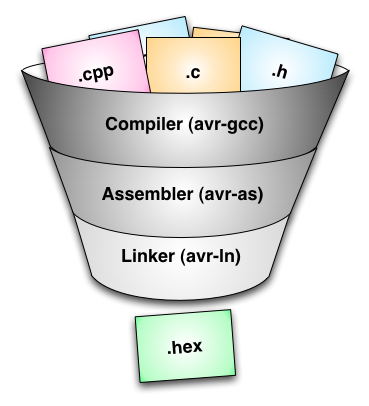
\includegraphics[width=0.26\textwidth]{avr}
\caption{An overview of the AVR toolchain}
\label{fig:tool}
\end{figure}
\begin{figure}[H]
\centering
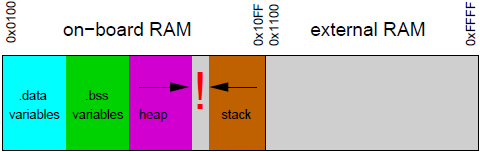
\includegraphics[width=0.48\textwidth]{ram}
\caption{The AVR / ATmega1281 standard RAM layout}
\label{fig:RAM}
\end{figure}
\subsection{AVR compiler}
\subsubsection{Toolchain Overview}
To develop software for an AVR microcontroller several tools are working together. This group of tools produces the final executable and is commonly called a toolchain and is shown in figure \ref{fig:tool}. 
\paragraph{GCC:} AVR uses the open source GNU Compiler Collection (GCC) with AVR microcontroller as target system. This version of GCC is known as 'AVR GCC' \defcitealias{AVR}{AVR-Libc User Manual, 2008}\citepalias{AVR}. GCC differs from other compilers, it only focuses on translating high level language to target assembly. For AVR GCC there are 3 language options: C, C++ and Ada. 
\paragraph{GNU Binutils: }The next step is done by another open source project called GNU Binutils. This contains the GNU assembler and GNU linker.
\paragraph{AVR-libc:} GCC and Binutils provide the tools to make the machine code but one critical component they do not provide is the Standard C Library. The open source AVR toolchain therefore comes with its own open source C Library project which contains many of the same functions found in the regular Standard C Library. It also adds many additional library functions that are specific to  AVR microcontrollers.
\paragraph{GNU Make:} Finally all pieces must be tied together. This is done by Make, which interprets and executes the Makefile of the project.
%------------------------------
\subsubsection{Memory Sections}
\label{memory}
The available non-volatile memory sections are the \textbf{.text} section (FLASH), which contains the actual machine instructions and the \textbf{.eeprom} section. Many AVR devices have a minimal amount of RAM. This limited amount of runtime memory needs to be shared between the following memory sections:
\begin{enumerate}
\item All initialized variables and static data such as\\ \verb+char message[] = "An error message"+ or \verb+USB.println("Another message")+ are stored in \textbf{.data variables}
\item Uninitialized global or static variables: \textbf{.bss variables}
\item Dynamic memory: \textbf{heap}
\item Area used for calling subroutines and storing local variables: \textbf{stack}
\end{enumerate}
The standard RAM layout is shown in figure \ref{fig:RAM}. Since there is no hardware supported memory management, separate regions can overwrite each other. Heap and stack can collide if either of them require large memory space or even when the allocations aren't high at all but because heap allocations get fragmented over time and new request don't fit in freed areas.\\ %figure was here
As discussed in section \ref{memory} the ATmega1281 is uses a modified Harvard architecture, meaning that data can also be stored in program memory space. This is useful when you have constant data and you're running out of room to store it. Remember that many AVRs have limit amount of RAM to store data, but may have available FLASH space left. For the compiler this is however a challenge, which is exacerbated by the fact that the C Language was designed for Von Neumann architectures. So the AVR compiler has to use other means to operate with these separate address spaces (cf. pointer usage). The AVR toolset used the GCC \verb+__attribute__+ keyword, which is used to attach different attributes to function declarations and variables. AVR GCC provides a special attribute called \verb+progmem+ for data declarations and tells the compiler to store the data in Program Memory. To increase the convenience to the end user AVR-libc provides a simple macro \verb+PROGMEM+ which can be found in 'avr/pgmspace.h'. To read the data another macro is provided, which generates the correct address to retrieve the data from Program Memory. Storing data in Program Space incurs extra overhead in terms of instructions and execution time, but usually this is minimal compared to the space savings.\\
\subsubsection{Memory problems}
Libelium's Programming Style Guide warns its users about the amount of memory \verb+USB.print("Test message!")+ requires. The program memory increases due to the instructions and arguments (the chars) needed to print the string. Since also the message itself is stored in the \textbf{.data} section \defcitealias{AVR}{AVR-Libc User Manual, 2008}\citepalias{AVR}, precious memory is wasted. As a fix, Libelium recommends to do the following:
\usestyle{vs}
\includecode{mem1.cpp}
This however still uses both program and data memory and is only useful if one wants to print the same message in different parts of the program, so this is not really a solution. The only way to save RAM memory while printing messages is to hard code them on the stack by doing the following:
\usestyle{vs} 
\includecode{mem2.cpp}
A less cumbersome way would be to give the message and an address where to store the message as argument of a recursive macro which does this operation for us. However, standard C macros cannot simply split a string into characters. So the only ways to save RAM is to hard code the string as data or to store the string in Program Space and use the \verb+strcpy_P+ to copy the string to stack when it is needed. 
\subsubsection{Compiler bugs}
When combining all pieces of software discussed in section \ref{program}, the Waspmote failed after a few cycles. It appeared as if Libelium's \verb+sendXBee(packetXBee *)+ function had a constant memory leak of 302 bytes. However, after examining all the related functions it became clear there were no implementation errors. After putting the necessary \verb+USB.print(freeMemory())+ statements before and after \verb+free()+ instructions, we concluded the \verb+free()+ instruction at line 5252 of 'WaspXBeeCore.cpp' failed\footnote{Issue 857: avr-libc 1.6.4 dynamic memory (malloc, free) bug, available at \url{https://code.google.com/p/arduino/issues/detail?id=857}, confirms this conclusion}. This was avoided by introducing a stack variable instead of a heap variable.\\
Another bug we discovered is with the assignment operator. For example assigning a \verb+uint16_t+ stack variable, that was needed for some evaluation, to a global \verb+uint16_t+ variable also fails sometimes for no clear reasons. Instead of using the temporarily stack variable, we re-assigned the evaluation to the global variable.    

\subsection{Libelium IDE and API}
\subsubsection{Waspmote-IDE}
The Libelium IDE offers some advantages compared to using other IDE's. For example by using Eclipse it is possible to update programs that are to big thereby over-writing the bootloader. Then they must be sent back to Libelium to restore them. The Waspmote IDE does not allow this accident, so Libelium does not support using other IDE's in an official way so that there is no valid warranty if you've erased the bootloader.\\
%------------------------------------
\subsubsection{Waspmote-API}
\label{LibAPI}
To facilitate the programming Libelium offers a quite big API and after some exploring you are quickly started with it. The structure of the API is very simple, there is little to no inheritance\footnote{Have a look at the graphs available at \url{http://www.libelium.com/v11-files/api/waspmote/db/d09/WaspClasses_8h.html} to get a complete overview of the API structure}. In this section, the most important classes are indicated with a red box and are recommended to explore before starting future programming.
\begin{figure*}[htbp]
\centering
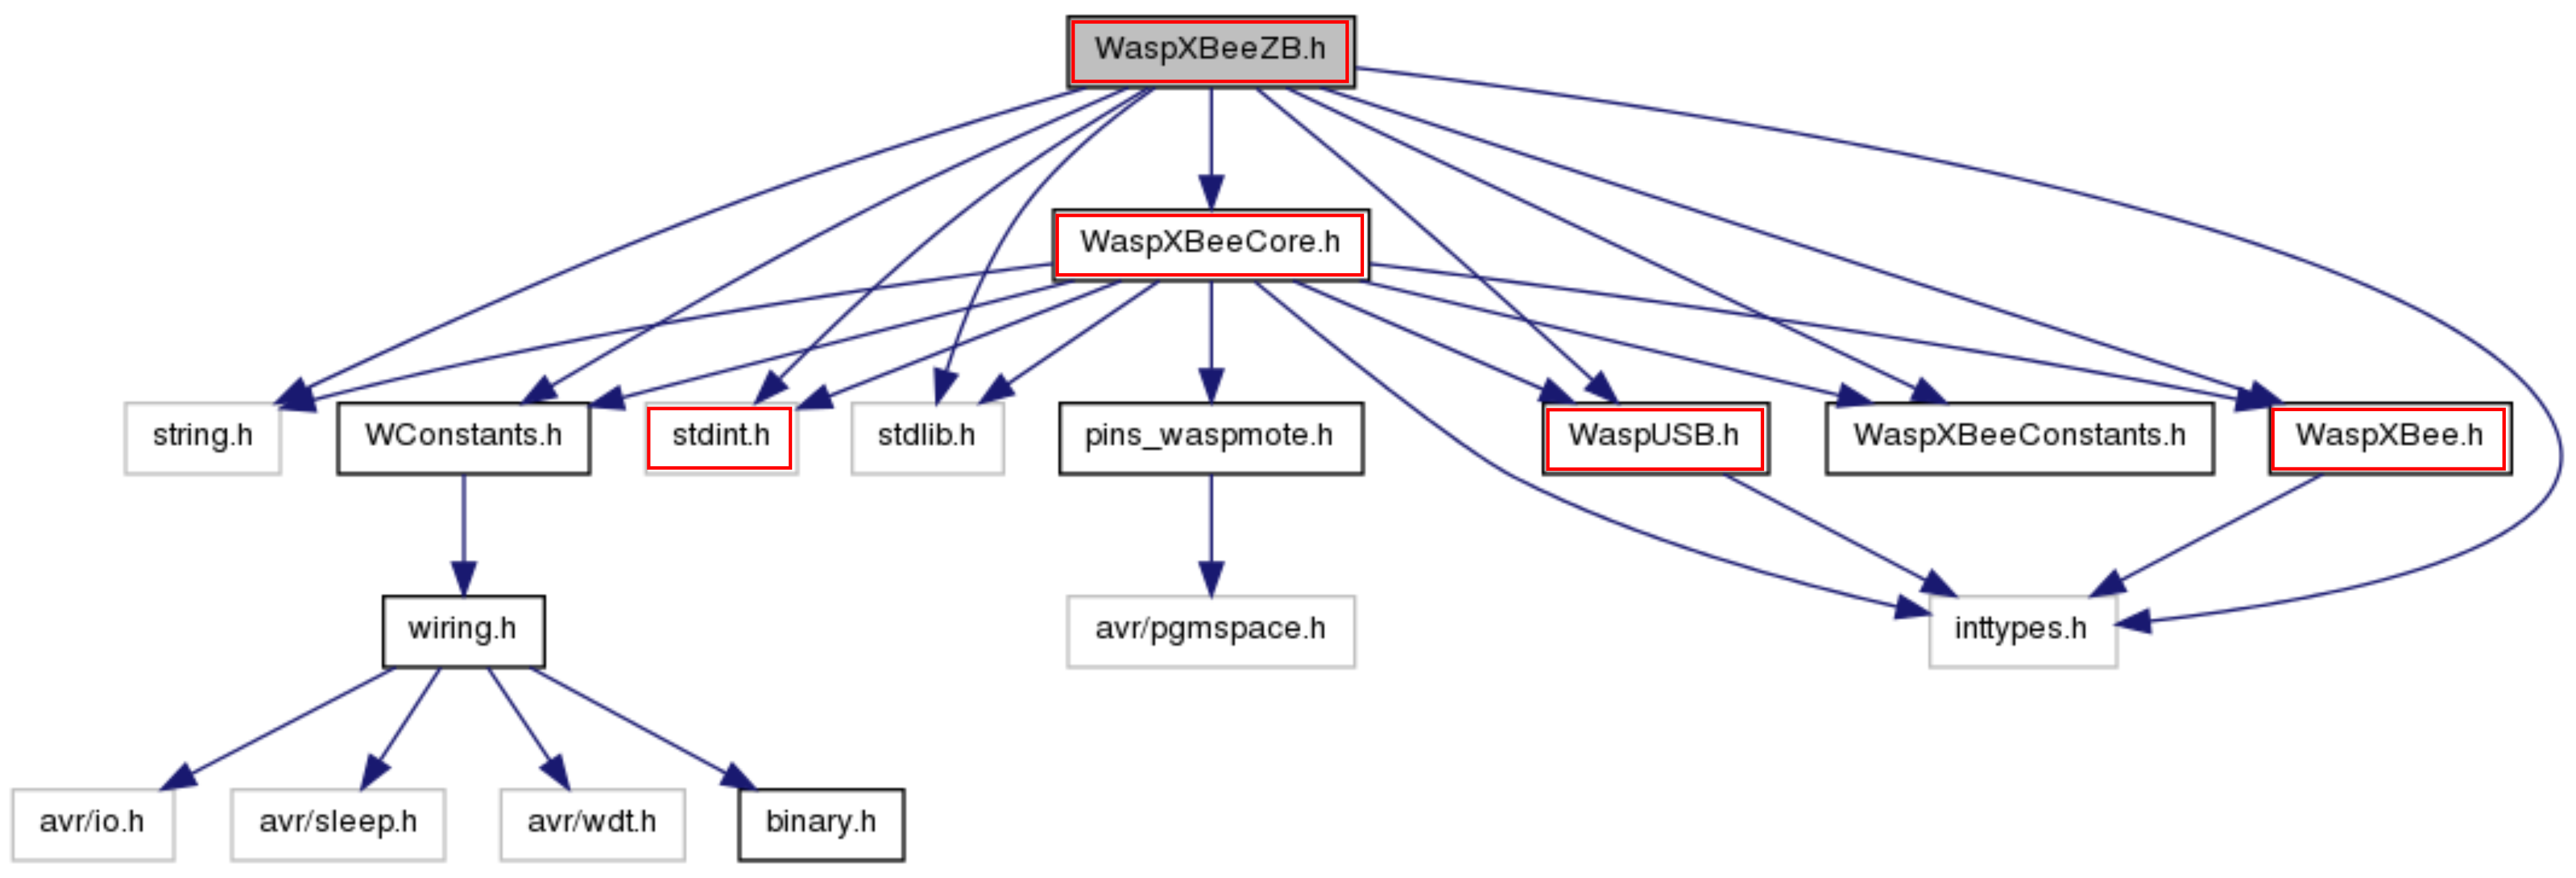
\includegraphics[width=0.98\textwidth]{API2}
\caption{Reduced dependency of Waspmote core libraries}
\label{fig:API2}
\end{figure*}
\paragraph{Original structure}
\label{object}
Each module or concept has its own class, for example all RTC functions are in 'WaspRTC.h' and 'WaspRTC.cpp'. To be able to use those functions in the IDE an object from the class 'WaspRTC' must be created. This object is created by default by the library and it is public to all libraries. All types to be run on the API can be found in the 'WaspClasses.h' file and each file also includes this file so it is aware of all available types.\\
For our application WaspXBeeZB is one of the most important classes. It inherits from WaspXBee Core and this way it is also related to the WaspXBee class. Figure \ref{fig:API2} displays the relationship with the AVR-libc libraries and the Waspmote hardware.\\ 
During the development of our program the Waspmote showed several strange effects that could only be explained by bad stack management or heap and stack conflicts. Because of this lack of free memory (SRAM, 8KB) we discovered that the V1.1 API wastes a lot of memory by always including all libraries, despite not using them. As a fix Libelium recommends via their forum to remove all classes you do not use, including there fields that are used in other classes, 'just' going through all the compiler errors one by one. After doing this our program had enough free memory and showed normal behaviour again.
%------------------------------------
\paragraph{Added functionality}
To facilitate programming extra functionality has been added to the Libelium API. They are inside files containing the original name with the 'Utils' addition, for example 'WaspRTCUtils.h' and can be found in 'BjornClasses.h'.
 
% Chapter 5

\chapter{Digital Signal Processor} % Main chapter title
\label{Chapter5} % For referencing the chapter elsewhere, use \ref{Chapter2} 
\lhead{Chapter 5. \emph{Digital Signal Processor}} % This is for the header on each page - perhaps a shortened title
\textsf{\textsl{Written by Bjorn Deraeve}}
%----------------------------------------------------------------------------------------
\section{Introduction}
\subsection{What is digital signal processing?}
Signal processing falls within the scope of electrical engineering and applied mathematics that deals with the analysis of signals or operations on signals. In order to do this signals are presented in descrete time, discrete frequency or other discrete signal domains. The set of algorithmic solutions that are used to process digital signals are limited by the processing capabilities of the available hardware. 
Digital Signal Processing (DSP) algorithms have long been run on standard computers. Today additional technologies such as specialized processors called Digital Signal Processors (DSP) are used. DSP processors can  perform typical DSP operations more efficiently thanks to single-cycle multiply-accumulate (MAC) units, shift registers and extra large accumulators. To increase speed and possible DSP realizations DSP processors are used in purpose-built hardware such as application-specific integrated circuits (ASICs) or field-programmable gate arrays (FPGAs).

%----------------------------------------------------------------------------------------

\subsection{How are DSP processors used?}
DSPs receive real-world signals like voice, audio, video, ... that have been diditized and then mathematically manipulate them. DSP processors are a special type of microprocessors which are designed for performing mathematical functions like "add", "substract", "multiply" and "divide" very quickly.
Real-world analog signals are converted by Analog-to-Digital converters and are turned into the digital format of 0s and 1s. Now the DSP can start working on this digitized information. When all processing is done the new samples are mostly feed back in the real world via Digital-to-Analog converters. This whole process happens at very high speeds.\\
\begin{figure}[htbp]
\centering
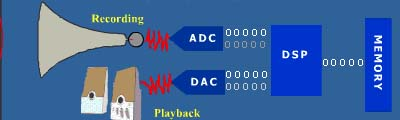
\includegraphics[height=3cm]{dspPrinciple}
\rule{30em}{0.5pt}
\caption{DSP Principle}
\label{fig:dspPrinciple}
\end{figure} \\
For our FM synthesizer application the first step is different. The DSP processing algorithms consist of algorithms that create the signal and signals that manipulate those signals so the AD converters on our FPGA are not used.

%----------------------------------------------------------------------------------------
\section{Digitization}  %sampling theorem
Real-world continuous signals have to be reduced to discrete signals (a numeric sequence) before a DSP can manipulate them. This sampling is done by an analog-to-digital converter (ADC) and the resulting samples are transported serially to the DSP.
\begin{figure}[htbp]
\centering
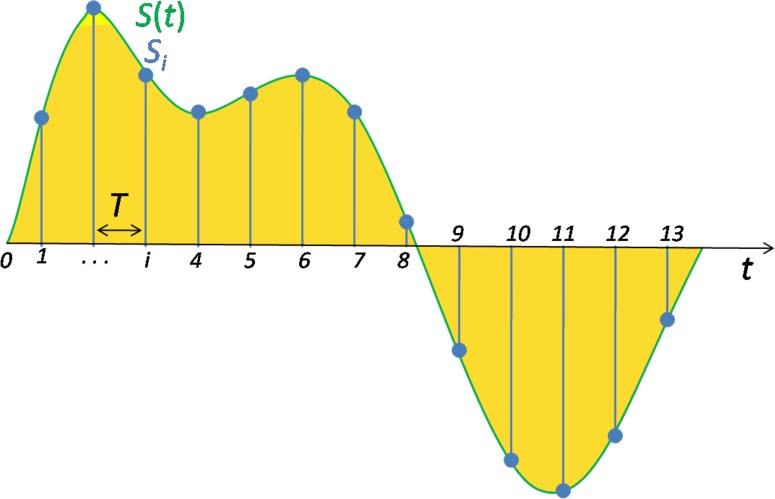
\includegraphics[height=3cm]{sampling}
\rule{30em}{0.5pt}
\caption{Signal sampling representation}
\label{fig:sampling}
\end{figure} \\
The sampling frequency $f_{s}$ is the number of samples taken in one second. According to the Nyquist criterion, the sampling frequency must at least be twice the frequency of the highest frequency component of interest. If the sampling frequency is greater than or equal to twice the bandwidth of a bandlimited signal then the signal can be (re)constructed without aliasing. This frequency is called the Nyquist rate. 
%----------------------------------------------------------------------------------------

\section{Digital Signal Processors}
As briefly mentioned in this chapter's introduction DSPs are processors with hardware, software, instruction sets, parallelism and data addressing that are optimized for high-speed numeric operations. 
A DSP contains the following key components:
\begin{itemize}
\item \textbf{Program Memory:} here the processing algorithms are stored
\item \textbf{Data Memory:} stores the signals to be processed
\item \textbf{Compute Engine:} performs the mathematical operations, coordinates access to program and data memory
\item \textbf{Input/Output:} connections to the outside world
\end{itemize}
\begin{figure}[htbp]
\centering
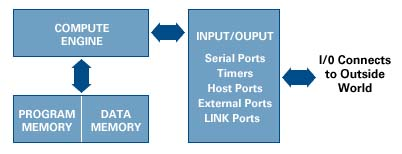
\includegraphics[height=2.5cm]{insideDSP}
\rule{30em}{0.5pt}
\caption[Structere of a DSP]{DSP structure}
\label{fig:insideDSP}
\end{figure} 
The need for high speed processors is because most DSP calculations are done on real-time signals. The inputsignal comes to the DSP as a train of individual samples from the AD converter. To do for example filtering in real-time, all calculations and operations on a sample must be completed before the next sample arrives. Usually also previous samples are needed so these must be stored somewhere and have to be quickly accesible. \\ 
%----------------------------------------------------------------------------------------
\subsection{Numeric architecture}
We know that DSPs must complete multiply-accumulate, additions and bit-shift operations in a single instruction cycle. Hardware optimized for such numeric operations is typical to DSP processors and distinguishes them from other general-purpose microprocessors.
The numeric operations are done by the DSP's MAC units, the arithmetic-logic unit (ALU) and barrel shifters:
\begin{itemize}
\item \textbf{MAC:} performs sum-of-products operations (used by FIR and IIR filters and fast Fourier transforms). The multiply-accumulate operation computes the product of two numbers and adds it to an accumulater:
\begin{equation}
a \shortleftarrow  a + ( b \times c )
\end{equation}
The multiplier is typically implemented in combinatonial logic followed by an adder and finally the accumulator register to store the result. If the output of the register is fed back to the adder each clock cycle the output of the multiplier is added to the register. Calculating multiplications with combinatorial logic requires a large amount of logic but is much faster than the method that uses shifts and additions.
\item \textbf{ALU:} performs standard addition, substraction and basic logical operations
\item \textbf{Barrel shifter:} performs operations on bits and words. This digital circuitry can shift a word by a specified number of bits in one clock cycle and is implemented as a sequence of multiplexers where the output of one mux is the input of the next mux. The input depends on the shift distance. An example of an 8-bit barrel shifter is shown in Figure \ref{fig:barrelShifter}. 
\begin{figure}[htbp]
\centering
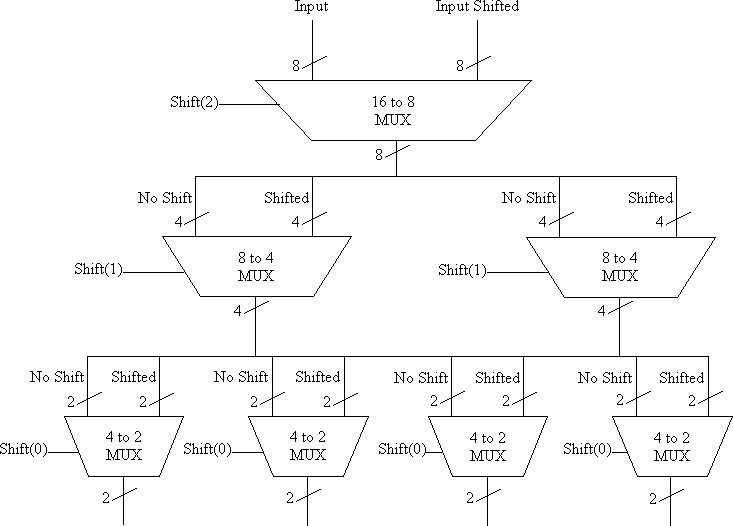
\includegraphics[height=6.5cm]{barrelShifter}
\rule{30em}{0.5pt}
\caption[8-bit Barrel Shifter]{8-bit barrel shifter}
\label{fig:barrelShifter}
\end{figure} \\
A barrel shifter is for example used for the implementation of floating-point arithmetic. To add two floats their significands must be aligned, which requires shifting the smaller number until it matches the exponent of the larger number.
\end{itemize}
As mentioned also parellelism plays a role in the efficiency of DSP processors. Figure \ref{fig:dspArchitecture} shows the parellelism of the ALU, MAC and shifter.
\begin{figure}[htbp]
\centering
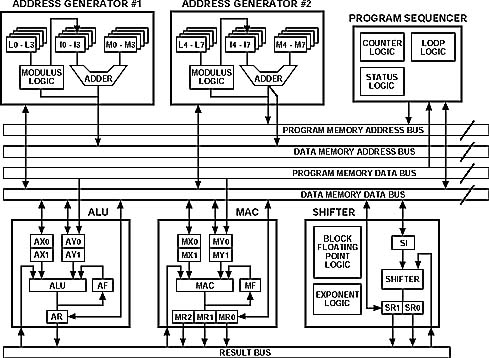
\includegraphics[height=6.0cm]{usefullDSPArchitecture}
\rule{30em}{0.5pt}
\caption[DSP architecture]{Useful DSP architecture}
\label{fig:dspArchitecture}
\end{figure}
%----------------------------------------------------------------------------------------
\subsection{Memory architecture}
Of course the memory of a DSP processor must be able to follow the high speed of the operations. Bus architecture must be optimized, there cannot be delays or bottlenecks. 
\begin{itemize}
\item Most general-purpose microprocessors use the von Neumann architecture and throughput is limited because of having to choose between either fetching data or fetching an instruction in each cycle. In DSP processors program memory and data memory have there own space and busses and can both be fetched in one cycle, doubling throughput. This structure is known as the Harvard architecture. Naturally additional optimizations  present on general-purpose processors, like instruction cache for example, are also present on DSPs.
\begin{figure}[htbp]
\centering
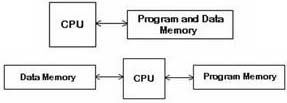
\includegraphics[height=2cm]{harvardVonNeuman}
\rule{30em}{0.5pt}
\caption[Harvard vs. Von Neuman]{Memory architecture: Von Neumann (top) vs. Harvard (below)}
\label{fig:harvardVonNeumann}
\end{figure}
\item A lot of DSP algorithms need to get data from memory in repeating patterns. For example the fetching and manipulation of samples stored in an array. By reducing instructions needed for memory access instruction cycles can be saved. To reduce this overhead DSPs use specialized data address-generators (DAG) to automatically manage these types of repeated memory accesses. 
Because most DSP algorithms use two operands the DSP has two DAGs. One address generator creates the address for the data memory bus, the other one for the program memory bus. By this way the DSP is able to sustain execution of instructions in one single cycle.
\item Often DSP algorithms require data in a range of addresses going from the end of the buffer back to the start of the buffer (wrap around). Therefore the DSP is provided with hardware circular buffers. The DAGs are specially designed for this task. General-purpose processors perform these functions in software and limit the ability to handle real-time signals.
\end{itemize}  
%----------------------------------------------------------------------------------------

\subsection{Sequencer architecture}
Since most algorithms runned on a DSP processor are by nature repetitive, the compute engine's program counter must be able to loop through the code without overhead while getting from the end of the loop back to the start. 
In general-purpose CPUs the loop's end condition is fully maintained in software. This condition instruction requires the fetching of addresses from memory and evaluation and takes time (cycles). DSP processors perform these tests in hardware, storing the needed addresses. In one cycle the condition is evaluated and either the first instruction of the loop is executed or the first instruction outside the loop is executed.
%----------------------------------------------------------------------------------------

\subsection{Input/Output architecture}
Because of the high data throuhput requirement of the DSP the whole design is focused on making data accessible for the numeric, memory and sequencer sections. To transfer data into and out of the DSP quickly serial communications and DMA is used. The use of serial communications above parallel is naturally since this way data is sended one bit at a time, following the DSPs operating frequency and distributing work load. So the DSP communicates with ADCs, DACs or other devices through synchronous serial ports (SPORT). Other functions such as timers and boot logic (in other words: hardware interrupts) also ease DSP system design. 
%----------------------------------------------------------------------------------------

\section{Fixed-point vs. floating-point DSP}
Digital signal processing can either be done with fixed point or with floating point data storage. DSPs designed to represent and manipulate integers are fixed point realizations. Floating-point DSPs represent and manipulate rational numbers. The number is represented in a similar manner to scientific notation, with a mantissa and an exponent (e.g. A $\times$ $2^{B}$ , where 'A' is the mantissa and 'B' is the exponent). 
\subsection{Advantages of floating-point digital signal processors}
In a fixed point DSP numbers are represented with a fixed number of digits after the decimal point, for example: 123.45, 1234.56, 12345,67, etc. In a floating point implementation the decimal point can 'float'.In addition a floating point representation can represent 1.234567, 123456.7, 0.001234567, etc.
Thanks to the exponential representation floating-point DSPs support a much larger dynamic range: very small numbers and very large numbers can be stored. Another advantage of this that floating-point processing yields much higher precision than fixed point processing.
\subsection{Considerations}
In digital signal processing rounding and/or truncating numbers yields quantization error or noise, a difference between the real-world value and the quantized digital values. This also happens each times a DSP does a mathematical calculation. As such, floating-point processors are the ideal DSP when accuracy is critical, like in audio applications. This is noticable in the program of our FM synthesizer, where constantly calculations are done with float data.
When choosing between fixed-point or floating-point processor there are many other important factors to consider, e.g. processor cost, ease of development, performance. In summary, because of the greater number of general purpose applications that can use fixed point processors those are typically less expensive than floating-point versions due to the scale of manufacturing. Floating-point DSPs are optimized for computationally intensive applications.
 
\section{Discussion}
WSNs can change everyone's life drastically and can be applied to many different areas. WSNs can help reduce CO$_{2}$ emissions for example. In a city where each parking space logs its occupation, a car can be guided to the nearest free spot. We have no doubt this technology has a bright future.
\section{Future Work}
The WSN Test-bed can be extended with the newer version of the Waspmote. Since the new Waspmotes provide an interrupt which enables the XBee to wake the Waspmote PRO, these ones should be used as end devices and the current versions should be used as routers.\\
In the preparation phase of this thesis we also created a simple XBee ZigBee module which runs on two AA batteries and is able to monitor a few sensors (see appendix \ref{mob}). Since these nodes are much cheaper than Libelium's hardware it would be nice if these nodes could also be integrated into the network. Unfortunately, because developing with the first generation Waspmotes took longer then expected, we could not test this any more. To realize this, one should extend the Libelium API with a function that is also able to read default API packets (without needing Libelium's extra application header).\\
At this moment, the test-bed will only accept request by authorized nodes (by default this is only the gateway). It would be a nice challenge to send the data encrypted as extra security. One must take in mind that this takes extra processor power and thus power consumption.\\   
The gateway has mostly been tested on a computer with plenty of memory and processing power. Optimizing this program for an embedded device is certainly possible. For instance, packets that could not be sent to Libelium are cached in memory. On embedded devices memory is limited so when memory is getting full these packets should be stored in a database until Ipsum is back online.\\
On the web service part it would be good to send a more detailed reply back to the client. Now only XML and URL are checked but if a node doesn't exist this is only detected in the main thread and the client is not notified of this error. The problem is that there are 20 threads to handle incoming requests. If the main detects a problem with a request it is hard to tell to which thread it should reply this problem since all the web service threads put packets in only one queue.\\
There is no way to communicate back to the client when something happens in the ZigBee network. If on Ipsum a sort of notification system could be installed where the gateway can put announcements or errors and the client would poll these announcements some more information about the status of the network could be delivered. For instance the pluvio sensor, which detects rain, works on interrupt basis. When this interrupt occurs for the first time in a longer period of time, we can assume it started raining. This could then be communicated back to the client trough an announcement. Or if the client requested an add node or add sensor but the ZigBee failed to reply in a certain amount of time it could be announced that this packet failed to deliver.\\
The program also has an SQL database. When this database fills up there is no strategy as what to when we run out of storage space. There are other and better database structures to deal with this.
 
\section{Conclusion}
During this thesis we successfully developed the WSN Test-bed, the gateway and the web client. To further expand the sensing capabilities of the WSN, we added a waterproof weather station mounted on a custom fitted stainless steel construction to guarantee long term operation.\\
For the ZigBee network the main challenges were power consumption and the responsiveness towards the users. To achieve low power consumption, long sleep periods are necessary, however this deteriorates the response time of the network. ZigBee has several good sleep options and supports wake on interrupt thus combining low power consumption with a high responsiveness. The first generation Waspmote does not support this, but the second generation does. By integrating the second generation Wasmpote PRO into the network, end devices can be made more responsive, increasing the overall network performance. ZigBee as a low power, low throughput networking protocol lives up to its expectations.\\
%Memory management on embedded devices is always a challenge. 
Also while developing the gateway different challenges were faced. Different services had to be connected to one another. Establishing the program structure required an iterative approach. Once this design was known, a decision had to be made on how to transfer information between the threads. We developed a lightweight solution using queues to achieve this. The gateway also provides certain features to avoid data loss. Since the gateway had to be multithreaded concurrency issues are avoided by using the necessary tools from the Boost library. Since the gateway is exposed to the outside world so that the client can access it, HTTPS is used as a safe means of communication. To verify the requirement that the gateway software can run on an embedded device, we successfully ported the program to a Raspberry Pi. This is a cheap solution in anticipation of a more permanent server.\\
The overall result is a controllable WSN test-bed in which new nodes and sensors can easily be integrated. Also the sensor data can be consulted in different formats via the web interface. This is the result of a good cooperation between all parties involved.

\section{Acknowledgements}
We would like to thank many people who have helped us with the completion of this dissertation. First of all we want to thank our supervisor, Luc Vandeurzen, for his guidance on technical as well as non-technical matters.\\
We are also thankful to Koen Pelsmaekers, who helped putting requirements together for the entire WSN, Ipsum and the web application project. To Ruben Tacq, who developed and helped us on our way with Ipsum.\\
We are beyond grateful to Matthias Verhelst, who worked on the development of the web interface for the WSN test-bed and for the cooperation in combining the different projects. To our parents for all there support, and especially Albert Deraeve, for transforming the weather station model into an exquisite construction.\\
Furthermore we would like to thank the people at Libelium for their advice on the Waspmote sketches.\\
Finally we want to thank Group T, for offering us the Libelium University Lab Kit and infrastructure to test and deploy our results.  
% Chapter 7
\chapter{Communication with LabVIEW User Interface using UART Port Controller} 
\label{Chapter7}
\lhead{Chapter 7. \emph{Communication with LabVIEW User Interface using UART Port Controller}}
\textsf{\textsl{Written by Thuy Pham}}
%----------------------------------------------------------------------------------------
\section{Introduction}
Communicating with peripheral devices plays a vital role in system design in general and in DSP systems specifically. For this purpose, SHARC Processor uses Digital Peripheral Interface (DPI). The interface provides both connections to two serial peripheral interface ports (SPI) and two universal asynchronous receiver-transmitters (UARTs). In this report, Universal asynchronous receiver transmitters (UARTs) will be examined in relationship with LabVIEW User Interface.\\
It is necessary to notice that the processor provide a full duplex universal asynchronous receiver/transmitter (UART) port, which is fully compatible with PC-standard UARTs. The UART port provides a simplified UART interface to other peripherals or hosts, supporting full duplex, DMA supported asynchronous transfers of serial data. The UART also has multiprocessor communication capability using 9-bit address detection. This allows it to be used in multi-drop networks through the RS-485 data interface standard. The UART port also includes support for five data bits to eight data bits, one stop bit or two stop bits, and none, even, or odd parity. More specifically, the UART port supports two modes of operation as mentioned below:
\begin{itemize}
\item \textbf{PIO (programmed I/O):} The processor sends or receives data by writing or reading I/O mapped UART registers. The data is double-buffered on both transmit and receive.
\item \textbf{DMA (direct memory access):} The DMA controller transfers both transmit and receive data. This reduces the number and frequency of interrupts required to transfer data to and from memory. The UART has two dedicated DMA channels, one for transmit and one for receive. This is the mode that will be used for transferring data between LabVIEW program and DSP board.
\end{itemize}
%----------------------------------------------------------------------------------------
\section{UART data frame}
\begin{figure}[htbp]
\centering
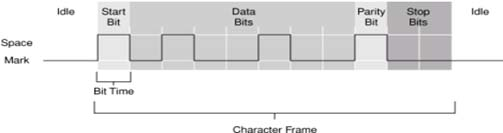
\includegraphics[height=3cm]{uart}
\rule{30em}{0.5pt}
\caption{A typical UART data frame}
\label{fig:uart}
\end{figure}
When two UARTs communicate, both transmitter and receiver need to know the signaling speed. The receiver does not know when a packet will be sent (no receiver clock); thus, the protocol is termed "asynchronous." This is very important because if we set up parameters (baud rate, start bit, stop bits, and parity bit) in both transmitter and receiver is incompatible, we will get incorrect data. In addition, the receiver circuitry is correspondingly more complex than that of the transmitter. The transmitter simply has to output a frame of data at a defined bit rate. Contrastingly, the receiver has to recognize the start of the frame to synchronize itself, and therefore determine the best data sampling point for the bit stream.\\ 
The processor supports a set of parameters' values for UART communication as below:
\begin{center}
\begin{tabular}[t]{|c|c|c|}
\hline
\textbf{SST} & \textbf{Parameters} & \textbf{Value}\\
\hline
1 & Baud rate & 2400, 4800, 9600, 19200, 38400, 57600, 115200, 921600, 6250000\\
\hline
2 & Data bits & 5 to 8 \\
\hline
3 & Stop bits & 1 or 2 \\
\hline
4 & Parity & None, even, odd \\
\hline
\end{tabular}
\end{center}
%----------------------------------------------------------------------------------------
\section{UART external interface}
The DSP processor communicates with peripheral devices in DSP board is described as the block diagram in figure \ref{fig:uart1}:
\begin{figure}[htbp]
\centering
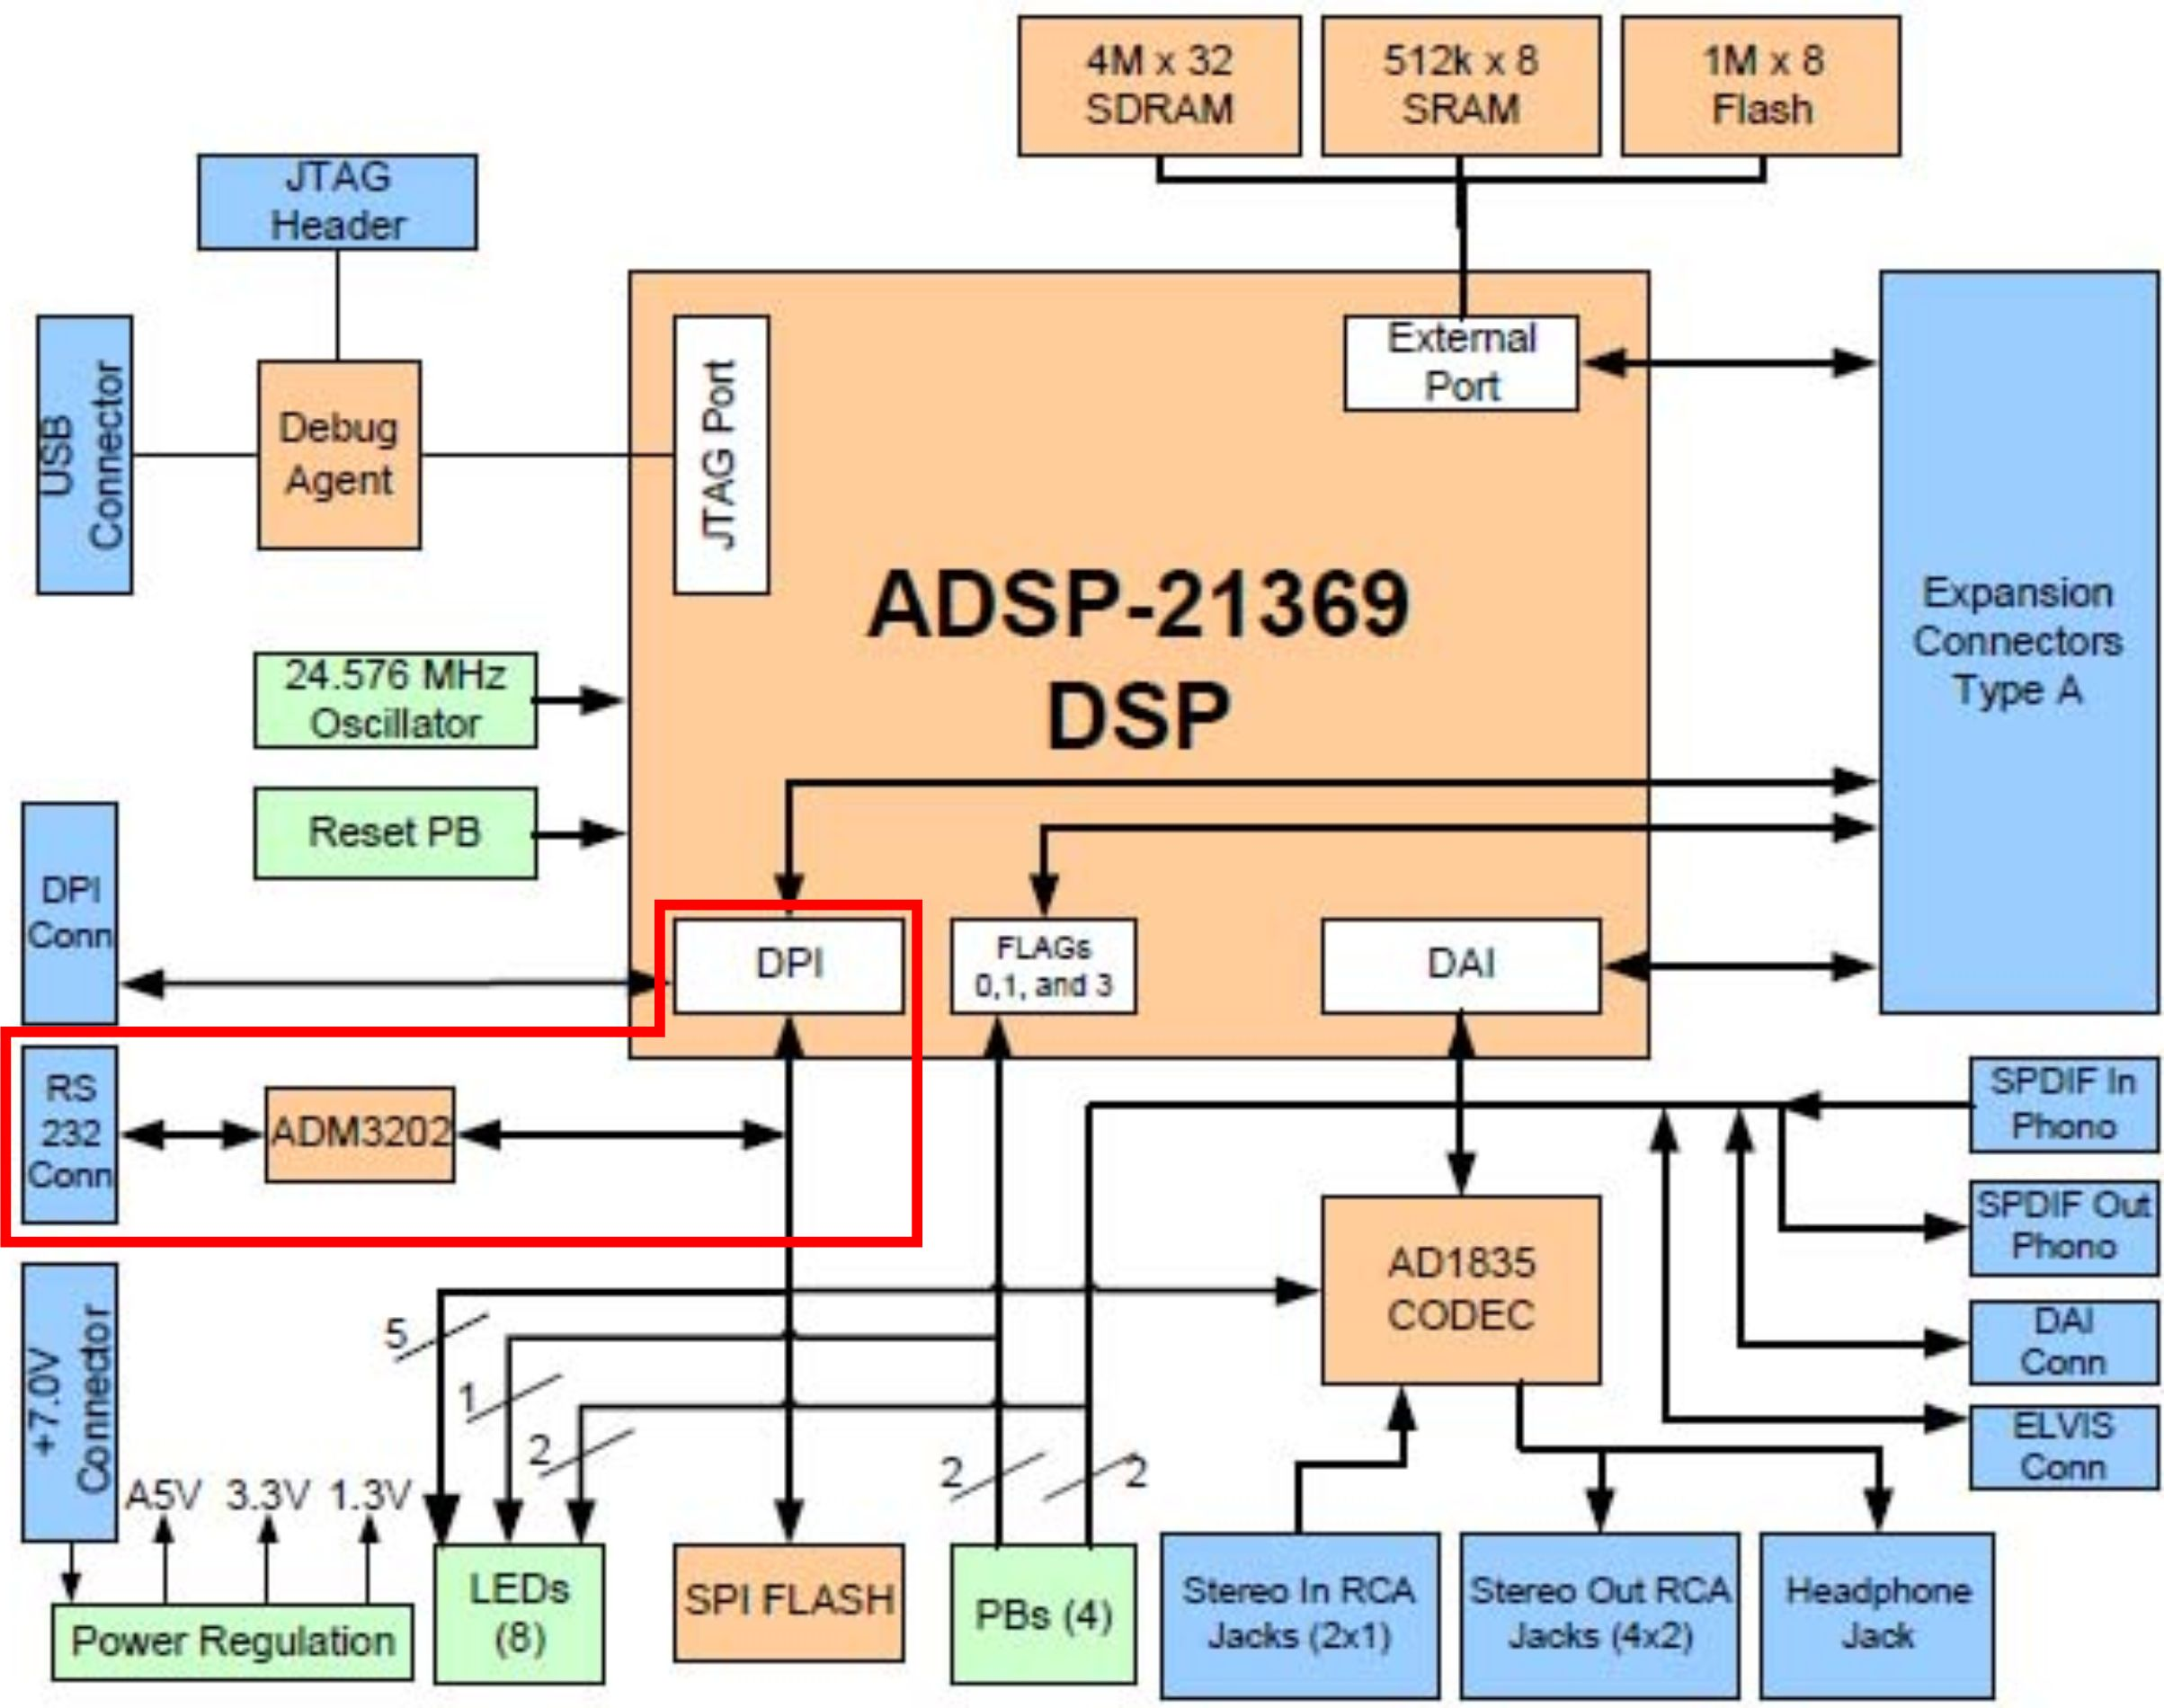
\includegraphics[height=8.5cm]{systemArchitectureDPI}
\rule{30em}{0.5pt}
\caption{System Architecture Block Diagram}
\label{fig:uart1}
\end{figure}\\
\begin{figure}[htbp]
\centering
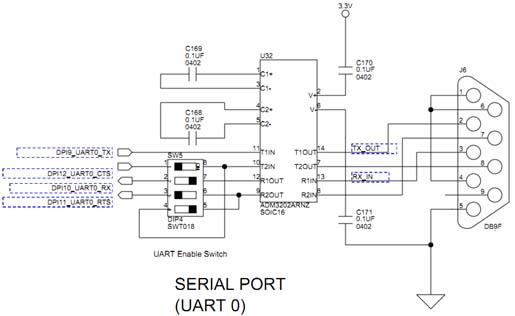
\includegraphics[height=6.5cm]{uart2}
\rule{30em}{0.5pt}
\caption{Schematic for connection of UART port}
\label{fig:uart2}
\end{figure}
In this board, the EIA-232E interface is used to communicate with other external serial communication devices. Instead of using traditional circuit for compatible purpose of power levels, in the DSP board, manufacture uses ADM3202 chip. The significant features of the chip are low power consumption and can operate at data rates up to 460 kbps make them ideal for battery powered portable instruments and high speed requirement.
%----------------------------------------------------------------------------------------
\section{UART configuration in DSP Processor for communication}
The DSP Processor provides a set of PC style, industry standard control and status registers for the UART.\\
\textbf{Register Overview for UART Module:}
\begin{itemize}
\item Line Control Register (UARTxLCR). Controls format of the data character frames. It selects word length, number of stop bits and parity.
\item Divisor Latch High/Low Register (UARTxDLL, UARTxDLH). Characterize the UART bit rate. The divisor is split into the divisor latch low byte (UARTxDLL) and the divisor latch high byte (UARTxDLH).
\item Mode Control Register (UARTxMODE). Controls packing and address modes.
\item Transmit Buffer Control Register (UARTxTXCTL). Controls core or DMA operation.
\item Receive Buffer Control Register (UARTxRXCTL). Controls core or DMA operation.
\item Interrupt Enable Control Register. Enables interrupt requests from system handling.
\item Line Status Register (UARTxLSR). Returns status of controls format of the data character frames as overrun or framing errors and break interrupts.
\item Transmit Status Register (UARTxTXSTAT). Returns status of core or DMA operations.
\item Receive Status Register (UARTxRXSTAT). Returns status of core or DMA operations.
\item Interrupt Identification Status Register (UARTxIIR). The register is used to get the status of all interrupts into one channel.
\end{itemize}
To configure parameters for transmitting data between PC and the DSP board, the number of simple steps can be followed:
\begin{enumerate}
\item \textbf{Route the UART to the DPI of DSP Processor}\\
The routing is implemented by software, in particular in the VisualDSP++, it is in the SRU macro. It is necessary to notice that, data is transmitted and received by the least significant bit (LSB) first (bit 0) followed by the most significant bits (MSBs).
\begin{figure}[htbp]
\centering
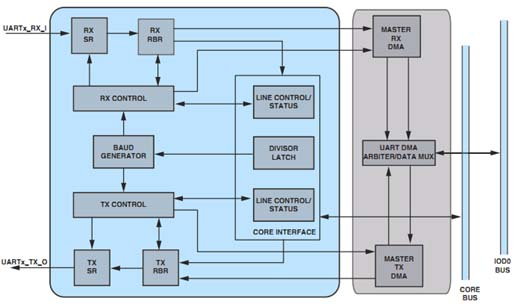
\includegraphics[height=6.5cm]{uart3}
\rule{30em}{0.5pt}
\caption{UART Functional Block Diagram}
\label{fig:uart3}
\end{figure}
\item \textbf{Set up baud rate, data bits, stop bits, parity bit}\\
The bit rate is characterized by the peripheral clock (PCLK) and the 16-bit divisor. The divisor is split into the UART divisor latch low byte register (UARTxDLL) and the UART divisor latch high byte register (UARTxDLH).  UART Baud rate = PCLK/(16 � divisor), where PCLK is the system clock frequency.\\
All data words require a start bit and at least one stop bit. With the optional parity bit, this creates a 7 to 12-bit range for each word. The format of received and transmitted character frames is controlled by the line control register (UARTxLCR).
\item \textbf{Set up core mode of operation}\\
This requires software management of the data flow using either interrupts or polling.\\
Core transfers move data to and from the UART by the processor core. To transmit a character, load it into the UARTxTHR register. Received data can be read from the UARTxRBR register. The processor must write and read one character at time. To prevent any loss of data and misalignments of the serial data stream, the UART line status register (UARTxLSR) provides two status flags for handshaking - UARTTHRE and UARTDR.\\
Core transfers through the UART is started by setting up and writing to transmit and receive control registers, enabling the module using the UARTEN bits in the UARTxTXCTL and UARTxRXCTL registers.
\item \textbf{Set up the UART interrupt}\\
The UART receive and transmit interrupts are programmed through the peripheral interrupt control registers (PICRx) as separate interrupts. (By default, these interrupts are not configured in the IRPTL register - the PICRx register has to be programmed to configure them.) \\
The UART interrupt enable register (UARTxIER) is used to enable requests for core system handling of empty or full states of UART data registers. When polling is used as a means of action, the UARTRBFIE and/or UARTTBEIE bits in this register are normally set.
\end{enumerate}
%----------------------------------------------------------------------------------------
\section{Programming for communication between DSP Processor and LabVIEW User Interface}
\subsection{LabVIEW program for writing data} \label{sec:Pham}
LabVIEW program provides a set of powerful tools for programming User Interface. Based on these things, user can make a program that clearly and visually shows parameters, graphs and results. LabVIEW also has many instrument drivers, which are a set of modular software functions that use the instrument commands or protocol to perform common operations with the instrument, for a variety of programmable instruments that use the GPIB, VXI, PXI, or serial interfaces.\\
With serial communication, in particular in RS-232, which is a standard developed by the Electronic Industries Association (EIA), LabVIEW provides some VISA functions for the target. They are located in \textbf{All Functions $>>$ Instrument $>>$ I/O $>>$ Serial}
\begin{figure}[htbp]
\centering
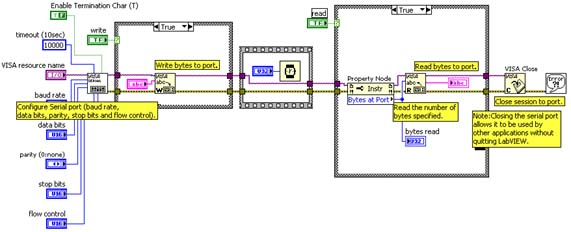
\includegraphics[height=6cm]{uart4}
\rule{30em}{0.5pt}
\caption{Write/Read a string to and from a COM port}
\label{fig:uart4}
\end{figure}
The VISA Configure Serial Port VI initializes the port identified by VISA resource name to the specified settings: timeout sets the timeout value for the serial communication; baud rate, data bits, parity, and flow control specify those specific serial port parameters.
\begin{enumerate}
\item The VISA Configure Serial Port VI initializes the port identified by VISA resource name to the specified settings: timeout sets the timeout value for the serial communication; baud rate, data bits, parity, and flow control specify those specific serial port parameters.
\item The VISA Write function sends the string.
\item The VISA Read function reads back up to bytes into the buffer, and the Simple Error Handler VI checks the error condition.
\item The VISA Close function terminates the communication channel to the instrument and deal locates the resources for the DSP.
\end{enumerate}
Depending on the purpose, the string can be written to the device in different forms. As the subVI described below, the string is combined by three parts, which are identified parameter order (two characters), the value needed to pass, and the character that uses for identifying read or write (character "w"). It is important to notice that maximum character transmission rate is depended on the baud rate and the bits per frame. More specifically, this rate is just the baud rate divided by the bits per frame. So, when there is a consecutive transfer required, the number of characters per string needs to be cared. Otherwise, there will be data lost.
\begin{figure}[htbp]
\centering
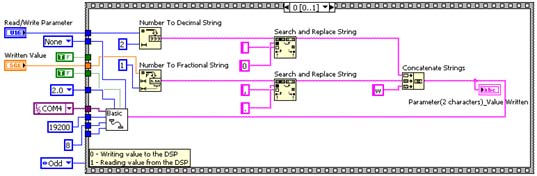
\includegraphics[height=4.8cm]{uart5}
\rule{30em}{0.5pt}
\caption{Formatting a string before writing to DSP}
\label{fig:uart5}
\end{figure}
Based on the prime subVI as showed in figure \ref{fig:uart5}, there are a number of ways to program an application that writes and reads multiple parameters to and from a DSP Processor. It needs to be reminded that, the principle of transferring data between DSP and PC is based on the interrupt. In other words, every time data is written to the DSP from PC, the serial DSP interrupt occurs and then its ISR (interrupt service routine) will run and process the received data. As a result, it is impossible to write more than one parameter at the same time that the DSP can process independently. Of course, each parameter has a different purpose. Because of this, the parameters should be organized so that only one parameter can write its data to the DSP at the time. It is very important for copying data between parameters that will be studied later.\\
Figure \ref{fig:uart6} shows an example program that wants to write multiple parameters to the DSP.\\
\begin{figure}[htbp]
\centering
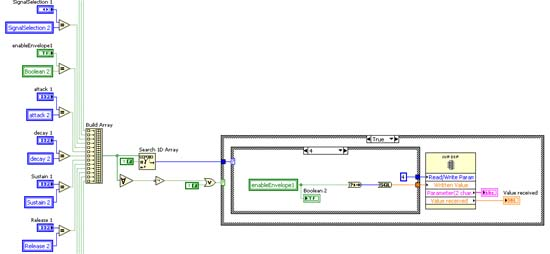
\includegraphics[height=6.6cm]{uart6}
\rule{30em}{0.5pt}
\caption{A part of writing parameters to Operator 1 program}
\label{fig:uart6}
\end{figure}\\
The idea of the program is that every time a parameter changes its value, which is detected due to search 1D array, the read/write part starts working. Otherwise, the program does nothing. This reduces a lot of works for the DSP Processor. Then, the latest value of the parameter and its order will be combined into string before writing to the processor. Notice that, LabVIEW also provides some data convert functions so that different data types of parameters can work properly.
%----------------------------------------------------------------------------------------
\subsection{UART Interrupt}
There are three things needed to be cared while using UART interrupts. First, you must map the UART interrupts to one of the interrupts in the interrupt vector table. In particular, the UART has to be mapped to exactly the peripheral interrupt sources. This can be achieved by changing the default source of the peripheral interrupt priority control register with the UART source, using the interrupt select values of the UART receive interrupt. The receive interrupt select values for UART0 (using in our application program) and UART1 are 0x13 and 0x14, respectively.
\begin{center}
\begin{tabular}[t]{|c|c|c|}
\hline
IIUART0RX & 0x3E00 & Internal Memory Address for UART0 Receiver\\
\hline
\end{tabular}
\end{center}
\begin{figure}[htbp]
\centering
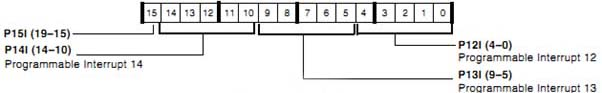
\includegraphics[height=1.5cm]{uart7}
\rule{30em}{0.5pt}
\caption{PICR2 Register}
\label{fig:uart7}
\end{figure}
\begin{alltt}
   *pPICR2 &= ~(0x3E0);  // Sets internal memory address for UART0 receiver
   *pPICR2 |= (0x13<<5); // Sets default value (0x13) for the URAT0 receive interrupt
\end{alltt}
The second thing is that enabling the UART interrupts internally by setting the corresponding bits in the UART interrupt enable register (UARTxIER). This needs to be done after all the UART settings (such as word length, parity, and so on) have been programmed, because in transmit mode as soon as the transmit buffer empty bit is enabled in the UARTxIER register, it vectors to the interrupt. If this bit is enabled before any of the UART settings are programmed, the data transmitted in the transmit interrupt service routine does not comply with the UART settings that are programmed later, leading to a communication error.
\begin{alltt}
   *pUART0IER = UARTRBFIE;   // Enables UART0 receive interrupt
\end{alltt}
The third, which is also the most important, is that using C Interrupt Handler with own Interrupt Service Routine. C provides its own set of interrupt handlers via the interrupt() and signal() functions. VisualDSP++ has extended the interrupt() function with \textbf{interruptf()} and \textbf{interrupts()} versions. The interrupt handler consists of three parts - the initialization, the interrupt vector, and the interrupt service routine. 
\begin{alltt}
   interrupt(SIG_P13, UARTisr);
\end{alltt}
Initialization performs the tasks previously associated with the C interrupt() function - assigning the interrupt service routine to an interrupt vector (dynamic ISR vectors only), unmasking the interrupt, and enabling global interrupts. The interrupt vector routes execution to the appropriate interrupt service routine. This routine must be compatible with the procedure of writing data of LabVIEW program. Otherwise, the data that DSP Processor expected to receive is different with data transmitted.
\begin{alltt}
   // Read the data from the buffer
   // Receive Buffer Registers (UARTxRBR)
      value = *pUART0RBR;
 
   /* Echoes back the value on to the hyperterminal*/
   // Wait until it is sent
      while ((*pUART0LSR & UARTTHRE) == 0)\{ ; \}

   // Writting a string to DSP
   // The character in buffer is "w" (ASC-II of "w" = 0x77 equivalent to 119 decimal)
      if(value == 119)
      \{
         for(i = 0; i < 2; i++)  address[i] = inputstream[i]; 
      
         // The two first characters writting from LabView is the index
         // int atoi(const char *str); - Convert string to integer 
            index = atoi(address);

         // The rest of the writting string is value (with a character - w)
         // Double atof ( const char * str ); - Convert string to double
         // 2 - is the place of starting value string 
            writtenValue = atof(inputstream + 2);

         // Writting value to the global variable
            algoparam[index] = writtenValue;    

         // Adds data to the buffer
         // Transmit Holding Registers (UARTxTHR)
            *pUART0THR = value;

            teller = 0;
      \}
\end{alltt}
%----------------------------------------------------------------------------------------
\subsection{The FM synthesizer application}
The application is programmed to provide two services. First, the program can write the values of parameters to the DSP so that DSP board can produce different sounds. Secondly, the LabVIEW User Interface also can show a number of features of the signal, such as the form of the envelope, frequency domain and the spectrogram.\\
To provide the features above, the application is programmed following a hierarchy as figure \ref{fig:uart8}.
\begin{figure}[htbp]
\centering
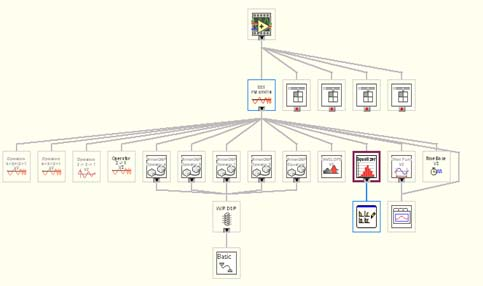
\includegraphics[height=5cm]{uart8}
\rule{30em}{0.5pt}
\caption{VI Hierarchy of LabVIEW User Interface}
\label{fig:uart8}
\end{figure}
\begin{figure}[htbp]
\centering
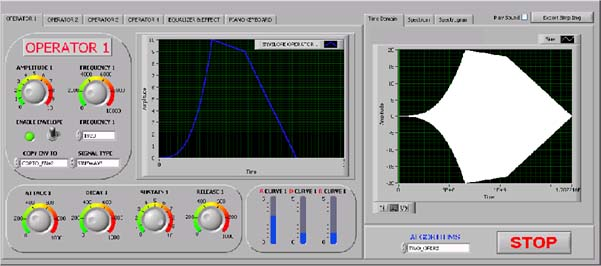
\includegraphics[height=5cm]{uart9}
\rule{30em}{0.5pt}
\caption{Front Panel of the application}
\label{fig:uart9}
\end{figure}
There are four main parts programmed in the application, which are programs for different algorithms of combining operators, programs for the envelope, programs for equalizer, sound effect and display, and writing data to the DSP board. The first part includes four algorithms: two operators, three operators, four operators modulated straightforward and four operators that actually consist of a pair of two operators. This part can be expanded in future to have more possibilities for producing sounds.
\begin{figure}[htbp]
\centering
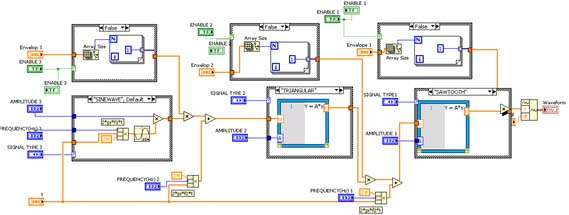
\includegraphics[height=5cm]{uart10}
\rule{30em}{0.5pt}
\caption{The algorithm for three operators}
\label{fig:uart10}
\end{figure}
The second part of the application is the envelope. It is used to modify the shape of the signal so that the output can have different frequency components. The third is programmed to produce more flexibility for the application. With this, user can choose specific range of frequency of the output signal (using the equalizer) and also can make distortion (using the effect part). The last one is writing data part, which is discussed in ''LabVIEW program for writing data", see section \ref{sec:Pham} above. More detail about the application, subVIs is available in appendix part in this report.
%----------------------------------------------------------------------------------------
\section{Conclusion}
This report discusses a number of things, which are needed to take into account when working with UART controller of the DSP processor and LabVIEW program. From my point of view, despite the fact that each part plays a different role to make the application work properly, the most important thing is that the data (a string of characters) need to be define completely the same in LabVIEW User Interface and UART interrupt service routine. Otherwise, the data that DSP Processor wants to receive for processing is not expected.\\ To improve quality of communication between LabVIEW User Interface and DSP board, context switch of UART interrupt needed to be considered. However, because of time and the limited ability, it could be studied in the future.
 
% Chapter 8

\chapter{Critical reflections} 
\label{Chapter8}
\lhead{Chapter 8. \emph{Critical reflections}}
\textsf{\textsl{Written by Bjorn Deraeve}}
%----------------------------------------------------------------------------------------
\section{Implementation problems}
In chapter \ref{Chapter6} we already explained how the program on the SHARC processor is designed. Here we will have a closer look at some problems encountered during the development.
\subsection{Communication with the Labview interface}
As explained in chapter \ref{Chapter7}, the parameters read from the interface are interrupt driven. As a consequence the program on the SHARC processor does not receive values if the user doesn't change any particular input on the interface.\\
For normal use this is not a problem since the values are initialized correctly when the program is started. However during the debugging process this often led to confusion and searching on problems in the code that actually weren't there.
%----------------------------------------------------------------------------------------
\subsection{Combining different program parts and general programming issues}
Including smaller topics like the envelopes, effects and equaliser into the main program sometimes led to major problems. Next to the inevitable minor adjustments in the program parts also the interaction with the interface caused problems. However, most of these problems were small mistakes that could easily be fixed. Nevertheless not all team members succeeded into fixing those little errors.\\
Sometimes it was necessary to change some details of the main program in order for the subprograms to work fluently. However, in order to do so efficiently one must at least understand the template we received at the beginning of the project and think well before changing stuff. There had to be intervened several times because a team member unknowingly stopped the whole program instead of just disabling his own algorithm. For example, as explained in chapter \ref{Chapter6}, processors on embedded systems need a \verb+while(TRUE)+ loop. Another useful thing to realize is that the periodic functions generating the waveforms need a variable that keeps track of the time. Updating this time in a local variable does not have the same effect like updating the global variable and again stops the program!\\
Also the modulo \%-operator is common in DSP algorithms and all team members should its meaning. Looking this up with google would have been a great idea!\\ Finally before asking to include a subprogram into the main program the smaller part must first have been debugged for syntax errors (since notepad doesn't highlight such errors).\\Next, some other concrete programming issues are described:
\begin{description}
\item[Sampling frequency:] The template we started from mentionned a sampling frequency of 48 kHz. However that project used a stereo audio channel which meant the samples were sent to the AD1835A at a rate of 96 kHz. Because we filled the algorithm's frames with mono channel samples (instead of two samples per calculation) our sampling frequency in software matched the sampling frequency of the hardware. \\ \\
\item[Modulation:] Enabling modulation caused some minor timing problems, however this could simply be fixed by passing the function's argument by value instead of by reference. \\ \\
\item[Envelopes:] There were several problems with the envelope. In a first stage nothing worked and a trick must be implemented to create envelopes with a duration longer than one second. To do so the function received a counter in its arguments. \\
The updating of this counter was at first done in the main synthesize sequence, when the program's time was an integer multiple of the sampling frequency. However because of the fixed frame length of 1024 samples this happend only every 4 seconds. To avoid this the updating of counter was originally moved to the create signal function. This has no influence and even made things worse actually. The problem with placing the flag here was that if modulation is enabled the flag updated several times. However this whole time the counter argument worked and the envelope refused working even without modulation.\\The underlying cause was that the envelope function made use of the wrong envelopes in memory so the parameters had no influence. Unfortunatelly not all team members were able to find such mistakes\\
Finally to fix all little problems the envelope received its own space in memory for keeping track of time. So now this isn't done anymore in the synthesize function but in the envelope itself. Because now the time is obviously updateted instaneously all problems are fixed. 
%\item[Envelopes, the bigger problem: ] There were several problems with the envelope. In a first stage nothing worked
\end{description}
%----------------------------------------------------------------------------------------
\subsection{Connecting the DSP board and use of the IDEs}
There were numerous of problems with Analog Devices' IDE. Personally I could not connect with the board on my normal Windows. Running the program from within a virtual machine on that same computer seemed to magically solve the problem (after a few years of internetting). If we have to invent an explanation I'd say that Sony tampered with the OS' USB drivers to make them more energy efficient and thus not supporting the DSP board.\\
Getting VisualDSP++ and Labview to run fluently also took a lot of time. For VisualDSP++ an activation code had to been registered. This became a problem since by the end of the project we got warnings that the activation would expend in less than a few days. Another issue with this activation code was that in week 10 a team member asked for it while it had already been e-mailed to all team members in week 4.\\
VisualDSP++ also seemed to be a very hard program to work with since a team member needed step-by-step click instructions for how to activate the editor's line numbers. \\
For Labview there were no valid licenses at all so the program had to be reinstalled a few times. Also to use all aspects of the interface several extra Labview plugins needed to be installed and again the only way to do is by completely reinstalling Labview, this became more or less a routine.
%----------------------------------------------------------------------------------------
\subsection{Extreme programming}
Due to the tricky situation with the interface several problems asked a lot of time to get fixed or didn't get fixed at all. For those harder to find errors a second pair of eyes would have been welcome.\\
Though in an attempt to improve the overal impression of the project it was best to do have look at those extra problems and happily been able to fix some of them. \emph{However it cannot be that there is only one person responsible to make all things work properly, the lack of a good programming partner was big. With such a partner a lot of improvements could have been made, some of them are discussed in section \ref{sec:future}.}
%----------------------------------------------------------------------------------------
\subsection{Latex}
Latex' standard color package does not support the color pink. My disappointment was huge, after heavy consideration I will declare this as the biggest lack encountered during this EE5-project.  
%----------------------------------------------------------------------------------------
\section{Team problems}
Next to common problems teams sometimes encounter like poor communication, group thinking and difficulty making decisions we also suffered from other problems. They are described shortly below:
\begin{itemize}
\item \textbf{Major issues}
\begin{itemize}
\item Lack of basic programming knowledge
\item Update files to the shared folder
\item Lack of inspiration for simple program features
\end{itemize}
\item \textbf{Minor issues}
\begin{itemize}
\item Update timesheets in time
\item Labview vs. C distinction
\item Give feedback on the programs: this only happened for the interface
\item Chaotic organisation of files in the shared folder
\end{itemize}
\end{itemize}
%----------------------------------------------------------------------------------------
\section{Achieved activities}
\begin{table}[hbp]
\begin{center}
\begin{tabular}[htbp]{| >{\centering\arraybackslash}m{4cm} | >{\centering\arraybackslash}m{4cm} |}
\hline
\textbf{Student} & \textbf{Hours}\\
\hline
Bjorn Deraeve & 210\\
\hline
Frederik De Greef & 140 \\
\hline
Kenneth Piot & 140 \\
\hline
Thuy Pham & 180 \\
\hline
\end{tabular}
\caption{Project logbook}
\label{tab:logs}
\end{center}
\end{table}
\begin{table}[!htbp]
\begin{center}
\begin{tabular}[!htbp]{|c|c|c|}
\hline
\textbf{Student} & \textbf{Topic}\\
\hline
Bjorn Deraeve & Admin: Meeting reports\\ 
& Labview: Connect the basic interface\\
& C: General program structure \\
& C: Signals and modulation \\
& C: Import and adapt (fix) the other programs\\ 
& C: Debug and fix envelope program\\
& Matlab: plots for report\\
& Labview: Bessel functions\\
& \LaTeX: cls, bib and tex template, chapters 1,2,5,6,8\\
\hline
Frederik De Greef & C \& Matlab: effects \\
& C \& Matlab: equaliser\\
& Report: chapter 4\\
\hline
Kenneth Piot & C: Envelopes \\
& Labview: Piano interface \\
& Report: chapter 2\\
\hline
Thuy Pham & Labview: full interface \\
& C: Configuration of UART communication \\
& Labview: waves and specta \\
& Labview: envelopes and graphs \\
& Labview: equaliser \\
& Labview: piano interface \\
& Report: chapter 7\\
\hline
\end{tabular}
\caption{Activities}
\label{tab:acts}
\end{center}
\end{table}
%----------------------------------------------------------------------------------------
\section{Future work}\label{sec:future}
This section summarizes some features that could add additional value to DSP Synthesizer.
\begin{description}
\item[Envelopes:] It is no coincidence the piano interface is located in the chapter on the envelopes. Combining the piano keystroke with the envelopes should have been an easy to implement extension.
\item[Equaliser:] An extended equaliser would provoke the musicians' creativity more.
\item[SDRAM:] Being able to save created sounds and reuse them to modulate signals. Also prestored effects could be offered this way. Search how to initialize the chip, \dots
\item[SHARC-ADSP 21369 IRQs:] Using the board's buttons to increase or decrease the volume. This is an interrupt driven event. Combining this interrupt with the other, time pressured interrupts, would have presented some interesting programming problems.
\item[Hardware controller:] Instead of using the labview interface use a real controller with a more advanced communication protocol. The board supports SPI, I$^{2}$C,\dots
\end{description}
 

%----------------------------------------------------------------------------------------
%	BIBLIOGRAPHY
%----------------------------------------------------------------------------------------

\label{Bibliography}

\lhead{\emph{Bibliography}} % Change the page header to say "Bibliography"

\bibliographystyle{ieeetr} % Use the "unsrtnat" BibTeX style for formatting the Bibliography

\addtocontents{toc}{\vspace{2em}}
%\clearpage
%\addcontentsline{toc}{\vspace{1em}}
\addcontentsline{toc}{chapter}{Bibliography}{\vspace{1em}}
\nocite{*}
\bibliography{./Bibliography} % The references (bibliography) information are stored in the file named "Bibliography.bib"




%----------------------------------------------------------------------------------------
%	CONTENT - APPENDICES
%----------------------------------------------------------------------------------------

\addtocontents{toc}{\vspace{2em}} % Add a gap in the Contents, for aesthetics

\appendix % Cue to tell LaTeX that the following 'chapters' are Appendices

% Include the appendices of the thesis as separate files from the Appendices folder
% Uncomment the lines as you write the Appendices

% Appendix A
\section{ZigBee Additions}%XBee join and send time experiments} % Main appendix title
\label{AppendixA} 

\subsection{ZigBee Stack}
\begin{figure}[htbp]
\centering
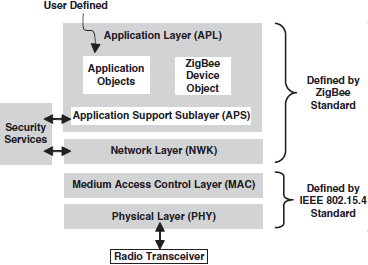
\includegraphics[width=0.58\textwidth]{stack}
\caption{ZigBee Protocol Layers ( $\circlearrowleft$ \ref{lab1} )}
\label{fig:stack}
\end{figure} 

%--------------------------------------------------

\subsection{Logical Device Types}
\begin{figure}[htbp]
\centering
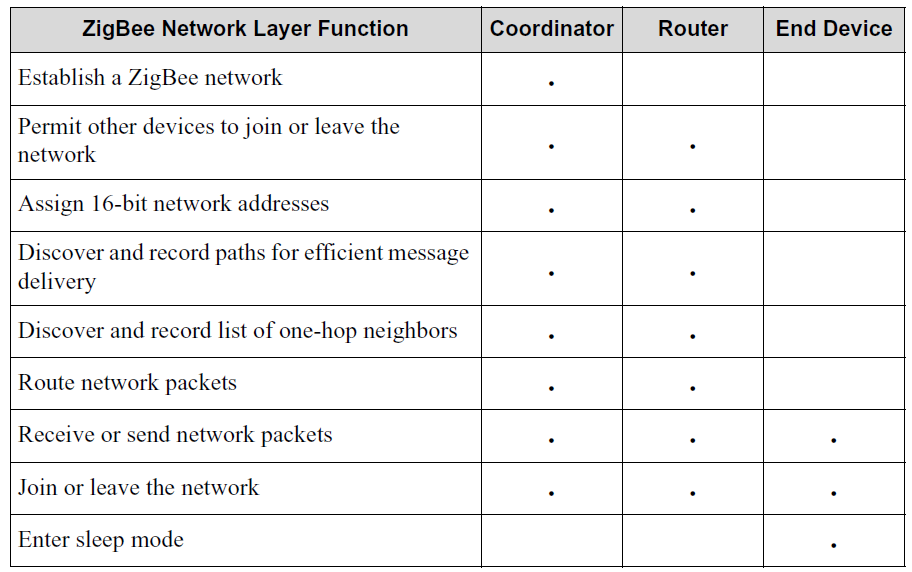
\includegraphics[width=0.78\textwidth]{roles}
\caption{Comparison of ZigBee Devices at the Network Layer ( $\circlearrowleft$ \ref{lab2} )}
\label{fig:roles}
\end{figure} 

%---------------------------------------------

\newpage
\pagebreak
\clearpage
\subsection{ZigBee Sleep Mode}
\label{zigbeesleep}
\subsubsection{Waspmote V1.1}
As mentioned in section \ref{lab5}, the current Waspmote program has the possibility to enable ZigBee / XBee sleep via the following definitions, accessible in 'PowerUtils.h' and the Libelium IDE, but will not use ZigBee sleep in default configurations.
\usestyle{vs} 
\includecode{sleep.cpp}

\noindent
This decision is based on the next conclusions related to the \verb+XBeeSleepMode+:
\begin{enumerate}
\item \textbf{Waspmote V1.1 has no support for wakening from ZigBee cyclic sleep}: When the Waspmote and the XBee are in sleep, the XBee should be able to wake the Waspmote when it detects his parent has a message pending for it. This is possible via a new interrupt routine added to Waspmote PRO. To do this on the first version one must solder pin 13 of the XBee to the MUX\_RX pin of the Waspmote. This way interruptions caused by the XBee module can be captured, but all other interruption options will be masked by pin 13's output and will thus be lost.
\item Enabling ZigBee sleep removes the association delay (see section \ref{second} ) but \textbf{requires 5 - 20 extra seconds to retrieve messages which are pending in the parent's buffer}. This has a very negative impact on battery life since all this time the XBee is turned on and receiving.
\item There is no guarantee that pending messages will be found when the Waspmote checks for them or in which order they will be received, so \textbf{network stability can no longer be guaranteed}. For example, when a privileged web interface user changes a sensor's measuring interval at minute 0 and another user re-changes the interval at minute 1, it is possible the request of the first user will be received after the request of the second user, so the node will not have the correct settings. This could be solved by adding timestamps to the requests or comparing the nodes responses with the web interfaces values. \item \textbf{Adding timestamps can help, however it is still possible that requests will go lost}. This happens from sleeping times of 15 seconds and more. This means that firstly the node will be much more active than sleeping. Secondly, the goal of using ZigBee sleep was to speed up the network response time and since packets can go lost due to enabling ZigBee sleep the network's response is worse than without using ZigBee sleep.
\end{enumerate}
\vspace{0.5cm}
\noindent
By checking for received messages immediately after sending sensor data, we can:
\begin{enumerate}
\item Guarantee network stability and disable ZigBee sleep
\item Save battery life by:
\begin{itemize}
\item Shorter duty cycles because we know when a message can be received
\item No XBee sleep current
\end{itemize} 
\end{enumerate}

%----------------------------
\subsubsection{Waspmote PRO} %to appendix
A sleeping Waspmote PRO can be interrupted when its sleeping XBee notices its parent has RF data available. The next paragraphs will briefly discuss the ZigBee protocol and settings.. 
\paragraph{ZigBee Sleep: Managing End Devices}
ZigBee end devices are intended to be battery powered and are capable of sleeping for extended periods of time. Because of this, routers and coordinators use packet buffers and transmission timeouts to ensure reliable data delivery to end devices.\\
When an end device joins the network, a parent-child relationship is formed with a router or the coordinator. From then on, if the end device is awake, it will send poll request messages (by default every 100 ms) to its parent to determine if the parent has any data buffered for it, independent of the sleep mode. Routers buffer this data only up to 28 - 30 seconds, so if we want to ensure reliable communication, this is the maximum sleep time. The child poll timeout can however be set up to a couple of months, so an end device can sleep longer than 30 seconds and still be considered to be in the network. This includes the node is associated within a few milliseconds, compared to the 2.5 seconds mentioned in section \ref{startup}. End devices can choose between two sleep modes, discussed in the next sections. 
\paragraph{Pin sleep}
In this mode an external microcontroller controls when the XBee should sleep and when it should wake by controlling pin 13. The module will not respond to serial or RF data when it is sleeping.\\\\
\textbf{+} lowest power consumption\\
\textbf{+} external controller can take samples without powering up the radio\\
\textbf{-} ZigBee protocol has less control\\
\textbf{-} external controller's timer is not accurate enough to synchronize the network\\
\textbf{-} Need fully awake parent\\
\paragraph{Cycle sleep}
Allows the XBee to determine when to wake up. The module can sleep for a specified time and wake for a short time to poll its parent for buffered data. If the parent has date the device will remain awake for a time, otherwise it will re-enter sleep mode immediately. 
\begin{itemize}
\item + suitable for DigiMesh, where the sleep clocks is accurate enough to get all nodes awake at the same time
\item + with DigiMesh, fully awake routers are not required, so they can be battery powered
\item - more power consumption due to accurate clock
\item - external controller must also wake when the XBee wakes to treat potentially received messages, even if there is no need to sample data
\end{itemize}

\paragraph{XBee sleep parameters}
\textbf{Router/Coordinator Configuration:} 
\begin{itemize}
\item RF Packet Buffering Timeout: 
\begin{itemize}
\item Sleep Period (SP) parameter. Max 30 seconds.
\item For cyclic sleep devices: SP should be set the same on routers and coordinators as it is on cyclic sleep end devices
\item For pin sleep devices: SP should be set equal to the time the end device can sleep, up to 30 seconds. If an end device sleeps longer than 30 seconds, parent and possibly non-parent devices must know when the device is awake. Therefore and devices that sleep longer than 30 seconds should transmit some kind of data (API frame) to alert the other devices that they can send data to the end device.
\end{itemize}
\item Child Poll Timeout: Sleep Number (SN) parameter: The number of Sleep Periods (SP) used to calculated end device poll timeout.
\end{itemize}

\vspace{0.5cm}
%--------------------------------------------------------------------
\subsection{Sleeping Mesh}
What is \textit{really} low power about ZigBee? The answer is already deducible from the previous sections, namely End Devices! A sleeping mesh tries to establish a multi-hop mesh network and low power routing functionality in one system, also using battery-powered routers. The system has two big requirements however:
\begin{itemize}
\item very low bandwidth, high latency
\item static network
\end{itemize}
For example, delivery of one data packet from every node every 12-24 hours, with a wake period of about 15 seconds. In a sleeping mesh all nodes wake up simultaneously and periodically to exchange and or route data. Afterwards, all nodes except the coordinator go back to sleep, a state which they are in 99\% of the time. In such a set-up battery lifes of 10 years and more are easy to reach.
\vfill
\pagebreak
%--------------------------------------------------------------------
\subsection{Range Test}
This procedure describes the easiest way to perform a range test using X-CTU. The test requires one coordinator node and one router node configured in AT mode.\\

\begin{enumerate}
    \item Set the target module address in both radios, as indicated in figure \ref{range1}.
    %\item To discuss digital systems of this scale and level of complexity
    %we need a number of descriptive tools.
    %\item For example:                                                 
    \begin{itemize} %label=\alph*)]
        \item item Module A will have the address of B in its destination field.\par
        \item Module B will have the address of A in its destination field. \par
        \begin{minipage}{\linewidth}
            \centering
            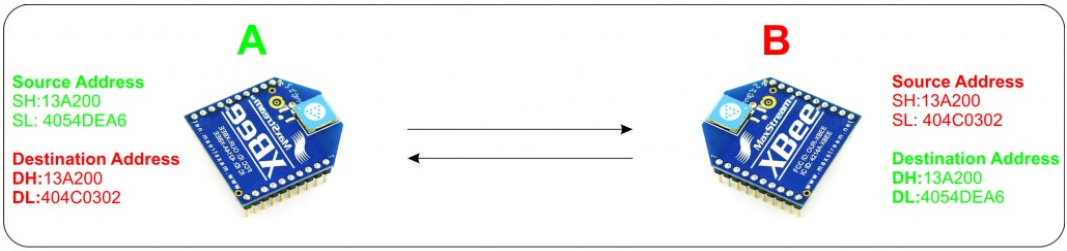
\includegraphics[width=12cm]{range1}
            \captionof{figure}{XBee Address Exchange}
            \label{range1}
        \end{minipage}
        %\item Timing diagrams highlight the detailed time sequence of
        %transfer between registers.\par
        %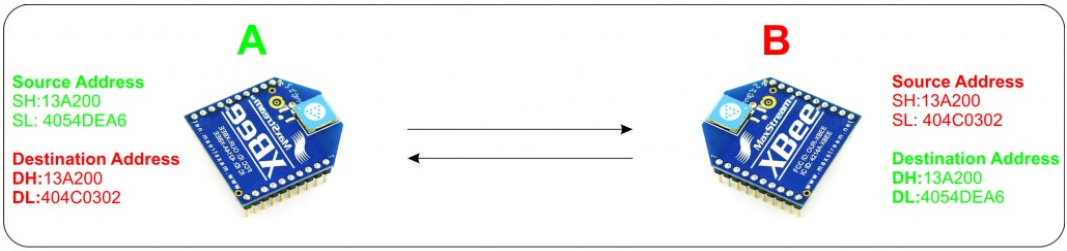
\includegraphics[width=10cm]{range1}
    \end{itemize}
    \item Make sure the modules have the same PAN ID and CHANNEL settings and write the values to the XBees.
    \item To do the range test, a data packet will be send and the module expects the same packet to be received:
	\begin{itemize}
		\item Connect the sending module to your laptop, e.g. module A. \par
		\item Module B must not be connected to any device but its Rx and Tx pin (XBee pin 2 and 3) must be connected to each other in order to create the loopback connection. To do this you can use a small breadboard. See figures \ref{range2} and \ref{range3}. \par
        \begin{minipage}{\linewidth}
            \centering
            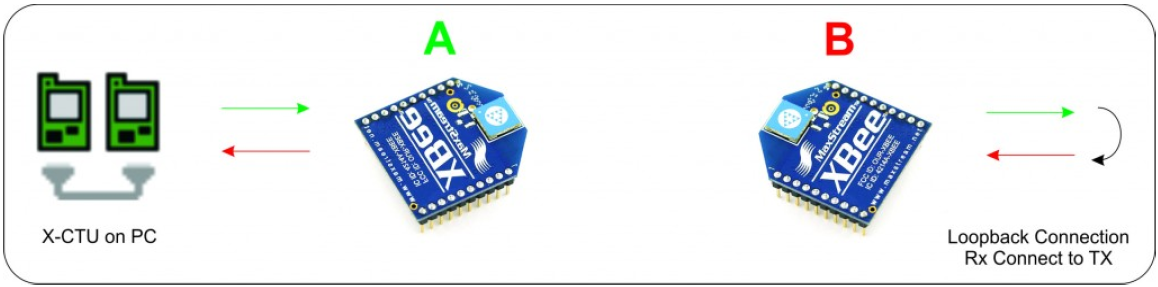
\includegraphics[width=12cm]{range2}
            \captionof{figure}{XBee Loopback Test}
            \label{range2}
            \vspace{1cm}
            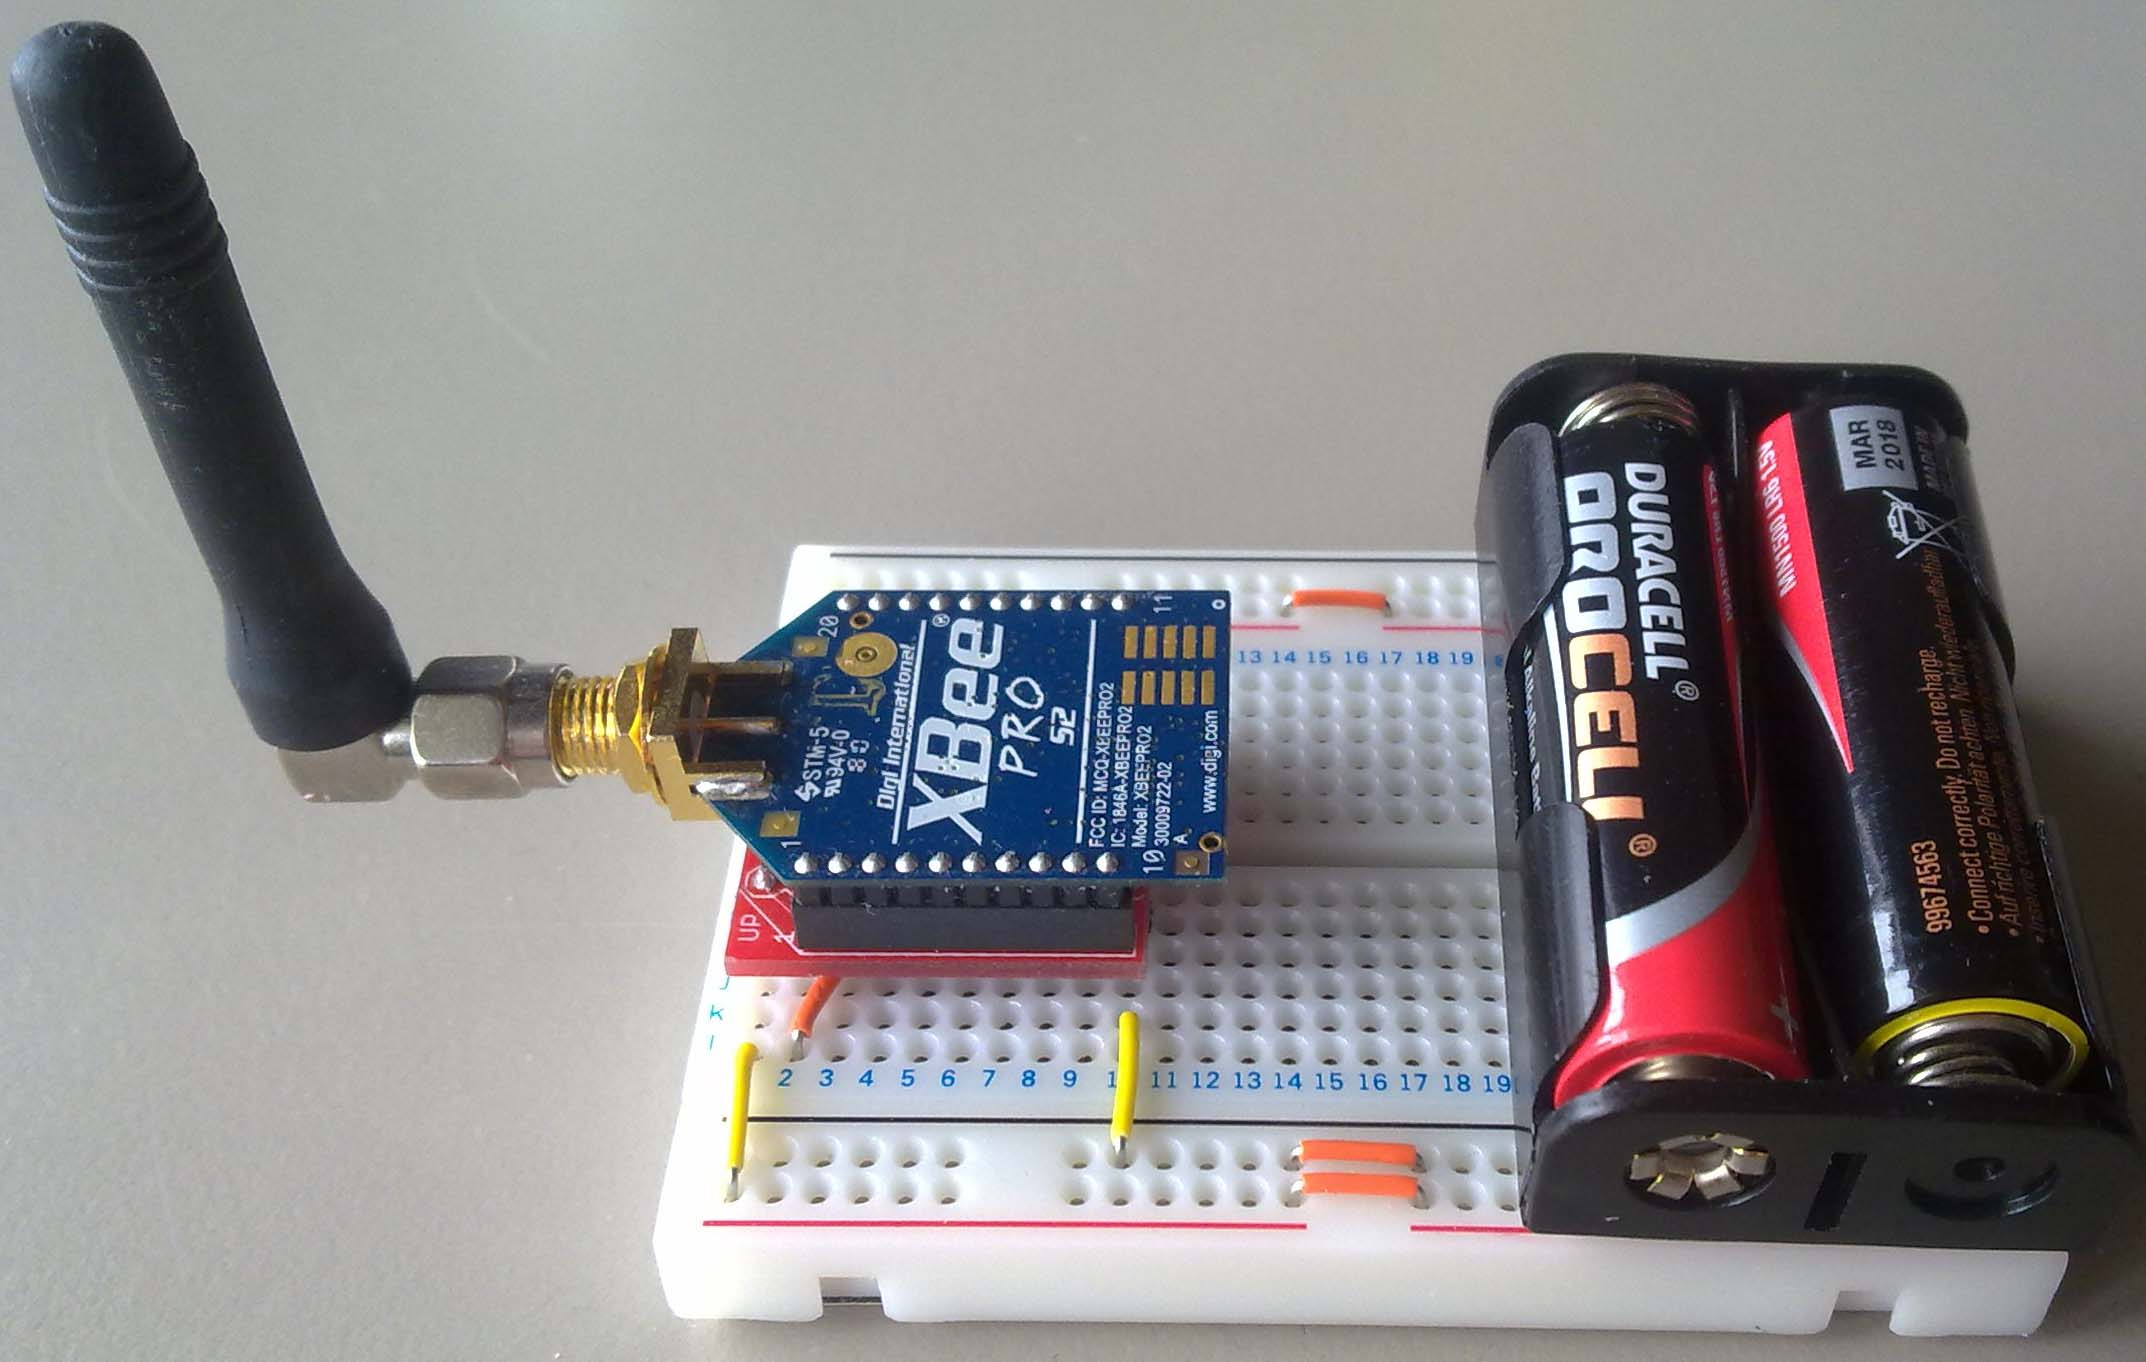
\includegraphics[width=12cm]{range3}
            \captionof{figure}{Module B Loopback Connection}
            \label{range3}
        \end{minipage}		
     \end{itemize}
     \vfill
     \pagebreak
     \item Go to the \textit{Range Test} tab in X-CTU, \textbf{select the checkbox under RSSI} and click \textit{Start} to run the test. Leave module B at a fixed position and walk around with your laptop to immediately see the RSSI value. Your screen should look as indicated in figure \ref{range4}. \par
             \begin{minipage}{\linewidth}
            \centering
            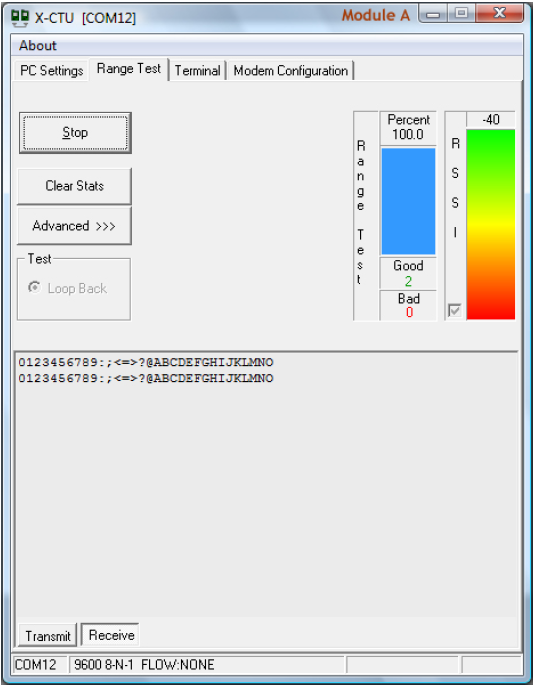
\includegraphics[width=10cm]{range4}
            \captionof{figure}{X-CTU Range Test}
            \label{range4}
        \end{minipage}
\end{enumerate}

\vfill
\pagebreak
\subsection{Self-made mobile XBee ZigBee node}
\label{mob}
\begin{figure}[htbp]
\centering
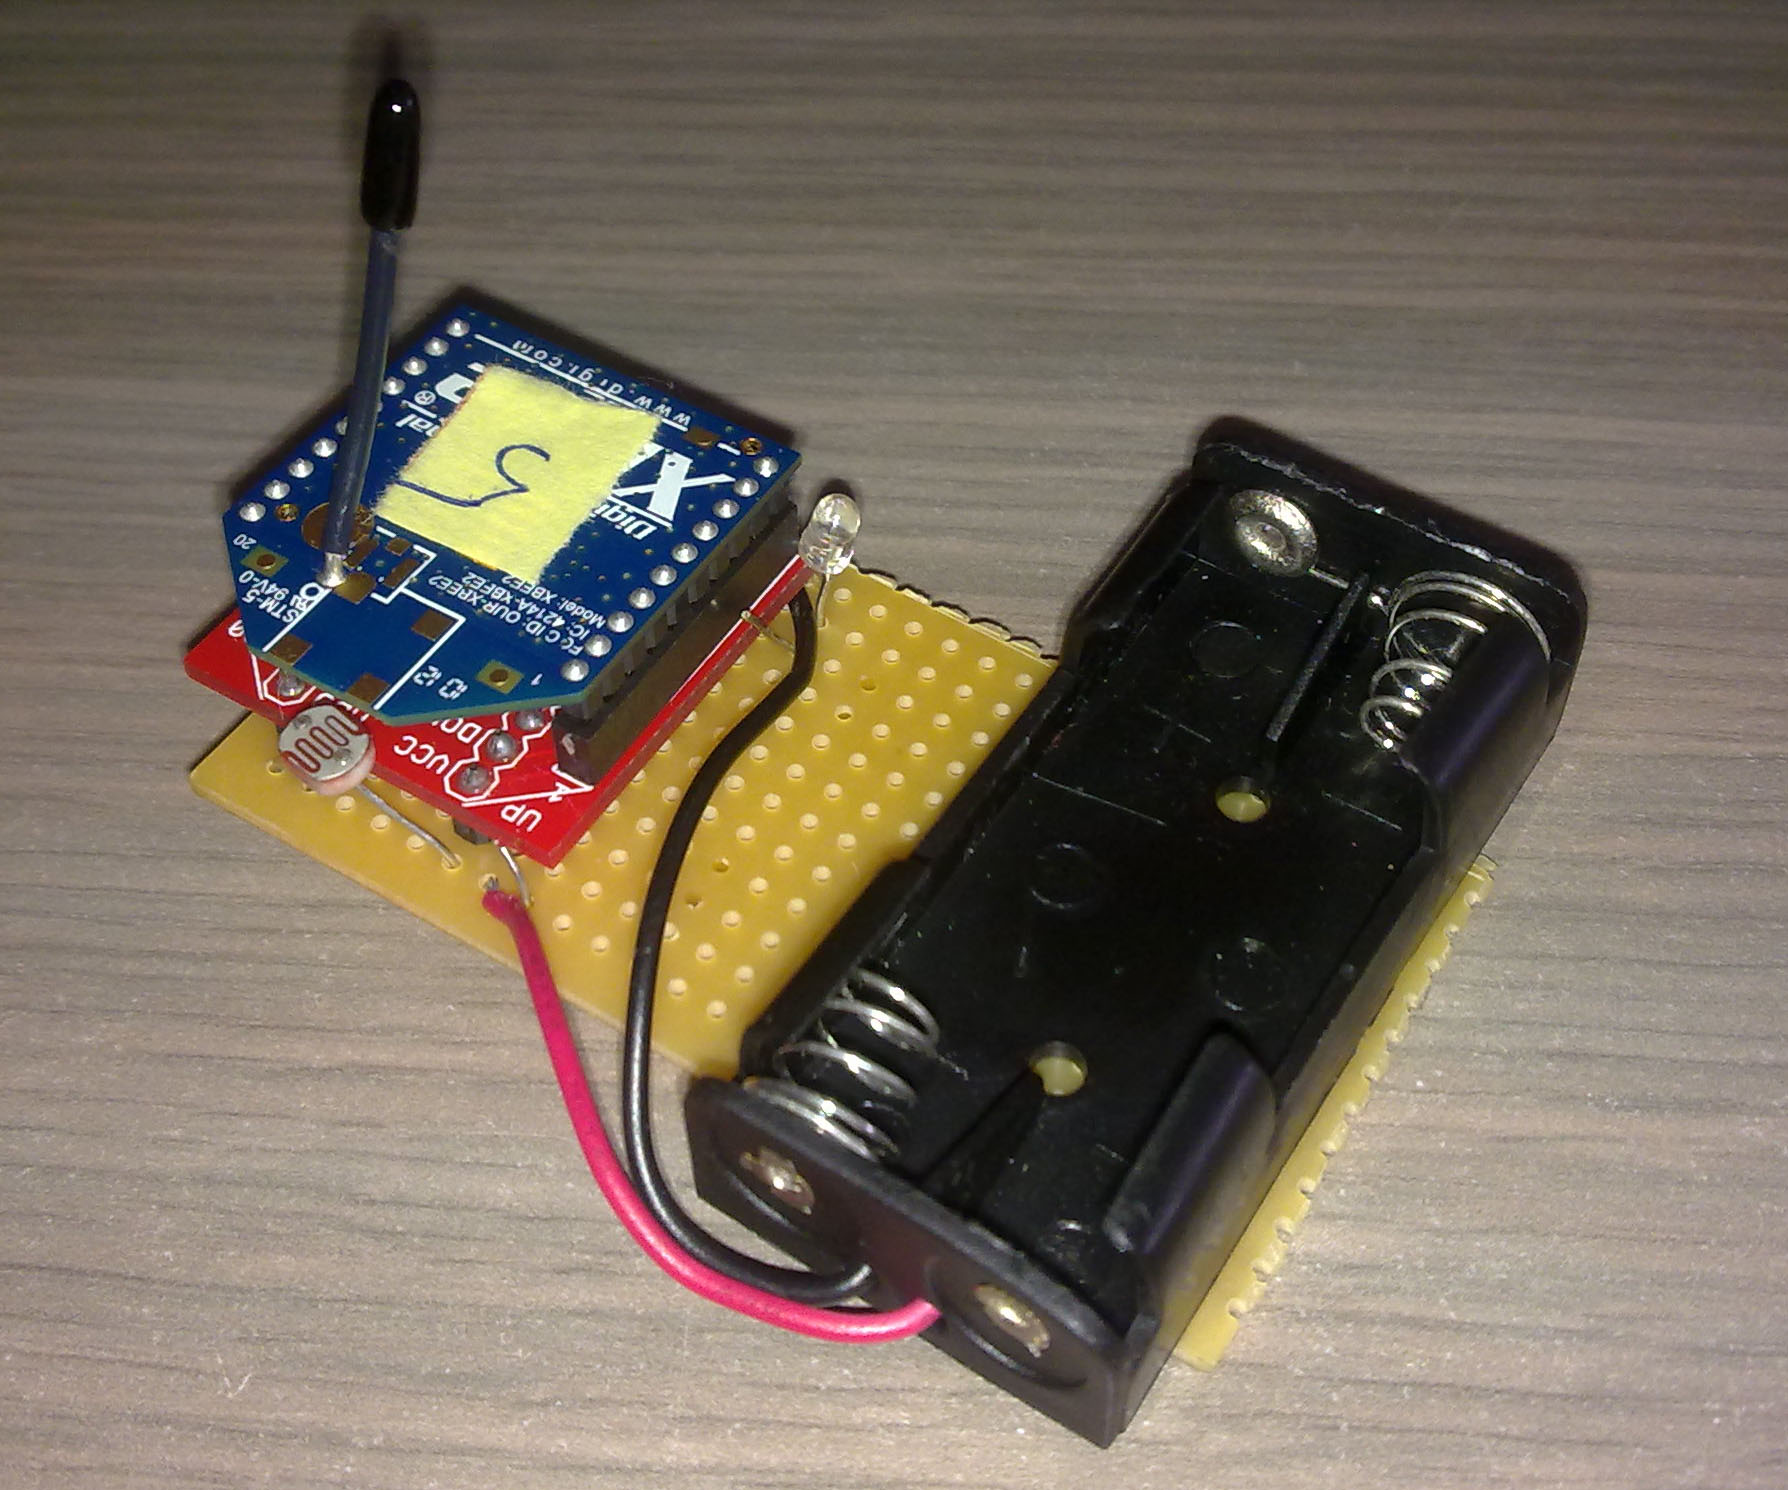
\includegraphics[width=0.78\textwidth]{mob}
\caption{A simple mobile node}
\end{figure} 
%input{./Appendices/AppendixB}
%% Appendix C
\newpage

\pagebreak
\clearpage
\section{Waspmote Variable Sleep Algorithms}
\label{AppendixC} % For referencing this appendix elsewhere, use 
\begin{table}[!hb]
\begin{center}
\begin{tabular}[!hb]{|c|c|c|c|c|}
\hline
\textbf{Sensor[4]} & \textbf{Sensor[3]} & \textbf{Sensor[2]} & \textbf{Sensor[1]} &\textbf{Sensor[0]}\\
\hline
100  & 50 & 35 & 10 & 20\\
\hline
\end{tabular}
\caption{Individual Sensor Sleep Times in seconds}
\label{tab:sleep1}
\end{center}
\end{table}
\begin{table}[!ht]
\begin{center}
\begin{tabular}[!ht]{|c|c|c|c|c|c|c|}
\hline
\textbf{Cycle} & \textbf{Sensor[4]} & \textbf{Sensor[3]} & \textbf{Sensor[2]} & \textbf{Sensor[1]} &\textbf{Sensor[0]} & \textbf{Sleep time}\\
\hline
0 & 100 & 50 & 35 & \textbf{10} & 20 & 10\\
\hline
1 & 90 & 40 & 25 & \textbf{10} & \textbf{10} & 10\\
\hline
2 & 80 & 30 & 15 & \textbf{10} & 20 & 10\\
\hline
3 & 70 & 20 & \textbf{5} & 10 & 10 & 5\\
\hline
4 & 65 & 15 & 25 & \textbf{5} & \textbf{5} & 5\\
\hline
5 & 60 & \textbf{10} & 20 & \textbf{10} & 20 & 10\\
\hline
6 & 50 & 50 & \textbf{10} & \textbf{10} & \textbf{10} & 10\\
\hline
\end{tabular}
\caption{Example of sleep algorithm 1}
\label{tab:sleep2}
\end{center}
\end{table}
%% Appendix C
\pagebreak
\section{Waspmote Battery Life Analysis}
\label{AppendixD} % For referencing this appendix elsewhere, use 
%--------------------------------------------------------------------
\subsection{High Performance Mode, without ZigBee sleep}
For this calculations it is supposed the batteries are in good condition and can be used with optimal conditions. The time values are taken from the third test scenario discussed in section \ref{second}, meaning that the Waspmote uses \textit{Hibernate} or \textit{Deepsleep} and the XBee is completely disconnected from the network.
The results are shown in figures \ref{fig:batCalcHP}, \ref{fig:batCalcHP1} and table \ref{fig:consump}.\\
%--------------------------------------------------------------------
\begin{figure}[htbp]
\centering
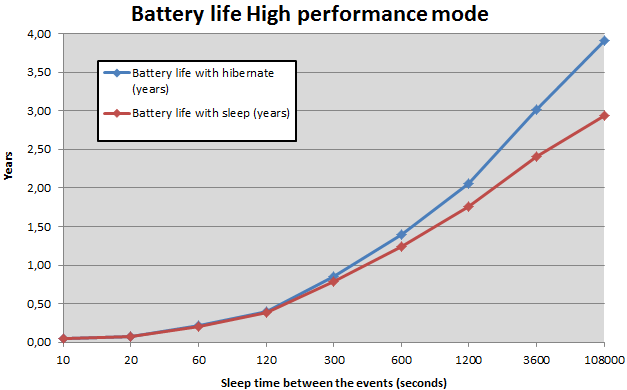
\includegraphics[height=8cm]{batCalcHP}
\caption{Battery life in High performance mode}
\label{fig:batCalcHP}
\end{figure}
%-----------------------------
\begin{figure}[htbp]
\centering
\includegraphics[height=8cm]{battery1}
\caption{Energy usage in High performance mode}
\label{fig:batCalcHP1}
\end{figure}
%-----------------------------
\begin{figure}[htbp]
\centering
\includegraphics[height=23cm]{cons1}
\caption{Energy usage in High performance mode}
\label{fig:consump}
\end{figure}
\pagebreak
%-------------------------------------------------------------------
\subsection{Power Saver Mode, without ZigBee sleep}
For these calculations Power Saver Mode is supposed. The Waspmote will switch on to measure sensors but not to send the data. The values will only be sent once every 60 samples, saving energy. The results are shown in figures \ref{fig:batCalcPS}, \ref{fig:batCalcPS1} and tables \ref{tab:sendTime3} and \ref{fig:consump2}. Finally table \ref{tab:cons2} summarizes the battery duration in years of both performance and power saver mode.\\
\begin{figure}[!ht]
\centering
\includegraphics[height=8cm]{battery2}
%\rule{30em}{0.5pt}
\caption{Battery life High Performance vs. Power Saver}
\label{fig:batCalcPS}
\end{figure}
%-------------------------
\begin{figure}[htbp]
\centering
\includegraphics[height=8cm]{battery3}
\caption{Energy usage in Power Saver mode}
\label{fig:batCalcPS1}
\end{figure}
%--------------------------------
\begin{table}[!ht]
\begin{center}
\begin{tabular}{cc|c||c|c|l}
\cline{2-5}
 & \multicolumn{2}{ |c|| }{Deep Sleep} & \multicolumn{2}{c}{Hibernate}\vline\\ \cline{1-5}
\multicolumn{1}{ |c| }{Sleep duration} & High Performance & Power Saver & High Performance & Power Saver    \\ \cline{1-5}
\multicolumn{1}{ |c| }{10s} & 0,05 & 0,92 & 0,05 & 1,00    \\ %\cline{1-5}
\hline
\multicolumn{1}{ |c| }{1min} & 0,21 & 2,15 & 0,21 & 2,63   \\ %\cline{1-5}
\hline
\multicolumn{1}{ |c| }{3min} & 0,79 & 2,75 & 0,85 & 3,59   \\ %\cline{1-5}
\hline
\multicolumn{1}{ |c| }{10min} & 1,25 & 2,85 & 1,39 & 3,76   \\ %\cline{1-5}
\hline
\multicolumn{1}{ |c| }{20min} & 1,75 & 2,90 & 2,06 & 3,85  \\ %\cline{1-5}
\hline
\multicolumn{1}{ |c| }{1h} & 2,41 & 2,94 &3,02 & 3,91    \\ %\cline{1-5}
\hline
\multicolumn{1}{ |c| }{3h} & 2,94 & 2,96 &3,90 & 3,94    \\ %\cline{1-5}
\hline
%\multicolumn{1}{ |c  }{\multirow{2}{*}{Powers} } &
%\multicolumn{1}{ |c| }{gcd} & 2 & 2 & 0 & 0 & min \\ \cline{2-6}
%\multicolumn{1}{ |c  }{}                        &
%\multicolumn{1}{ |c| }{lcm} & 3 & 3 & 1 & 1 & max \\ \cline{1-6}
\end{tabular}
\caption{Battery life in years for High Performance and Power Saver}
\label{tab:cons2}
\end{center}
\end{table}
%-----------------------------
\begin{table}[!ht]
\begin{center}
\begin{tabular}[!ht]{|c|c|}
\hline
\textbf{Nr of samples per sensor} & \textbf{Average ON time (ms)}\\
\hline
10 & 210\\
\hline
3 & 194\\
\hline
\end{tabular}
\caption{Time needed to sample and store 4 sensors}
\label{tab:sendTime3}
\end{center}
\end{table}
\pagebreak
%-----------------------
\begin{figure}[htbp]
\centering
\includegraphics[height=18cm]{cons2}
\caption{Energy usage in High performance mode}
\label{fig:consump2}
\end{figure}
%-------------------------------------------------------------------
\clearpage
\pagebreak
\subsection{High Performance vs. Saver Mode, with ZigBee sleep}
%% Appendix C
%\newpage
%\pagebreak
\clearpage
\section{Waspmote Flow Chart}
\label{AppendixE} % For referencing this appendix elsewhere, use 
\begin{figure}[htbp]
\centering
\includegraphics[height=18cm]{WSN2}
\caption{Flow chart of the Waspmote program for end devices}
\label{fig:flow}
\end{figure}


\addtocontents{toc}{\vspace{2em}} % Add a gap in the Contents, for aesthetics

\backmatter


\end{document}  
